\documentclass[output=paper]{langsci/langscibook}
\ChapterDOI{10.5281/zenodo.1407019}
\title{Les affixes dérivationnels ont-ils des allomorphes~? Pour une modélisation de la variation des exposants dans une morphologie à contraintes}

\shorttitlerunninghead{Les affixes dérivationnels ont-ils des allomorphes?}

\author{Fabio Montermini \affiliation{CLLE-ERSS, CNRS \& Université de Toulouse 2 Jean Jaurès} }

\abstract{Cet article traite des phénomènes de variation formelle en dérivation (écart entre la forme attendue et la forme réellement observée pour un lexème dérivé) qui ne peuvent pas être traités en termes de variation thématique, ce qui suggère que les exposants des constructions morphologiques peuvent à leur tour être sujets à variation. Pour modéliser cette variation des exposants, je propose d'étendre la notion de contrainte\is{constraint} non seulement à une propriété qui est spécifique à une langue donnée, mais également à une construction donnée. Les exposants des constructions morphologiques sont alors eux-mêmes vus comme des (ensembles de) contraintes\is{constraint} qui interagissent avec les autres contraintes\is{constraint} en jeu dans la formation des lexèmes complexes. Chaque «~allomorphe\is{allomorphy}~» d'un exposant est donc représenté comme une contrainte\is{constraint} qui, en tant que telle, peut être hiérarchisée par rapport aux autres, ce qui rend compte de l'observation que certaines de ces variantes jouent un rôle de défaut, alors que d'autres émergent uniquement dans des conditions particulières. Afin d'illustrer ce modèle, je propose deux études de cas de constructions morphologiques de naissance ou développement récent. Il s'agit, d'une part, de la création de noms de locuteurs en \emph{-phone} à partir du nom d'une langue et la création de lexèmes avec un sens génériquement appréciatif / superlatif en \emph{-issimo}. Chacune de ces deux constructions est à son tour comparée à des constructions proches: la dérivation en \emph{-phone} est comparée à la dérivation correspondante et cognate de lexèmes en \emph{-fono} en italien ; la dérivation en \emph{-issimo} est comparée à la dérivation, plus canonique, de superlatifs en \emph{‑issime} en français. Ces comparaisons mettent en lumière le fait que des constructions formellement et sémantiquement similaires et qui ont la même origine peuvent, dans des langues différentes ou dans la même langue à des époques et pour des finalités différentes, développer des spécifications phonologiques différentes, ce qui se traduit, dans le cadre adopté ici, par des ensembles de contraintes\is{constraint} différentes et/ou agencées différemment.
}

\maketitle

\begin{document}
\selectlanguage{french}
\il{French|(}
\il{Italian|(}
\is{allomorphy}

\section{Introduction}

Un des changements majeurs qu'a connus l'étude de la morphologie dans
les dernières décennies a été le glissement des modèles morphématiques,
décompositionnels et combinatoires vers des modèles davantage tournés
vers la description des relations existantes entre des mots plus ou
moins complexes. Une des conséquences de ce changement est le fait que
ces relations ne sont plus analysées en termes de règles orientées,
déterministes et existant indépendamment des unités qui les incarnent,
mais en ayant recours à des concepts comme celui de «~patron~» ou
«~schéma~», plus souples, et qui rendent compte de la manière dont les
locuteurs établissent des généralisations à partir du lexique existant.
C'est ce que l'on observe, par exemple, dans la Morphologie des
Constructions (\isi{Construction Morphology}), élaborée principalement par
%
%Booij (2010)
\citet{Booij10}%
%Booij
%
, mais aussi dans le modèle à contraintes\is{constraint}, élaboré par
%
%Hathout (2009) 
\citet{Hathout2009a} %
%Hathout
%
et surtout dans les travaux récents de Marc Plénat et
Michel Roché %
%(Plénat \& Roché 2014~; Roché et Plénat 2014, 2016)
\citep{Plenat-Roche2014,roche2014.CMLF,Roche16}%
%Plénat-Roché;Roché-Plénat;Roché-Plénat
%
. Toutes
ces approches sont «~output-oriented~», au sens qu'elles sont moins
intéressées à décrire l'ensemble de procédures qui permettent de passer
d'un input à un output (un lexème (plus) complexe) qu'à rendre compte
des contraintes\is{constraint} qui pèsent sur la forme (et le sens) d'un lexème
construit, ou, plus précisément, de tous les lexèmes construits qui
appartiennent à la même série (c'est à dire, qui sont construits par la même opération
morphologique). Parmi d'autres résultats, les approches en question ont
permis de rendre compte de manière efficace de la variation
allomorphique\is{allomorphy} observée dans le lexique construit, en particulier en ce
qui concerne la sélection du thème\is{stem} du lexème de base et les éventuelles
modifications qu'il subit. En revanche, à quelques exceptions près
%
%(notamment Lignon \& Roché 2011)
\citep[notamment][]{LignonStephanie2011}%
%Lignon-Roché
%
, la variation de forme des exposants
(celle qui est appelée traditionnellement l'allomorphie\is{allomorphy} affixale\is{allomorphy!affix allomorphy}) a été
peu discutée dans ce cadre. Une des raisons principales est certainement
le fait que les approches dont il est question ci-dessus ont le plus
souvent pris le parti de maximiser la complexité des représentations
lexicales en simplifiant, parallèlement, l'instruction phonologique
associée aux opérations morphologiques, et donc de repousser, autant que
possible, l'allomorphie\is{allomorphy} du côté des radicaux\is{stem} plutôt que du côté des
affixes (%
%Bonami \emph{et al.} 2009
\citealt{Bonami2009b}%
%
, par exemple, sont très clairs sur ce
point). Pourtant, le fait que l'allomorphie\is{allomorphy} puisse toucher aussi bien
les radicaux\is{stem} des mots construits que les affixes semble souvent aller de
soi, en lexicographie, dans plusieurs cadres phonologiques (par exemple
en Théorie de l'Optimalité), mais également pour la morphologie, que ce
soit la morphématique traditionnelle (ce qui est normal, puisque dans
ces cadres les radicaux\is{stem} et les affixes sont des objets de la même
nature) ou la morphologie lexématique dite «~classique~». Dans ce
contexte, une position emblématique me semble être celle de %
%Scalise (1999~: 457)
\citet{Scalise1999}%
%
, qui, en traitant des noms déverbaux de l'italien, se demande
«~in \emph{amministrazione} il suffisso sarà -\emph{azione},
-\emph{zione} o -\emph{ione}?~» (`dans \emph{amministrazione} le suffixe
est-il -\emph{azione}, -\emph{zione} ou -\emph{ione}~?'), en suggérant
simultanément qu'il est possible (et intéressant) d'identifier une forme
précise pour le suffixe dans le dérivé en question -- et par conséquent
d'établir une frontière nette entre le suffixe et le radical\is{stem} -- et que
celui-ci peut potentiellement se présenter sous de différentes formes.

\newpage 
Dans cet article je vais proposer, au contraire, qu'une question comme
celle ci-dessus n'est pas une question pertinente et que, si l'on se
place dans un cadre morphologique orienté vers les outputs et basé sur
les contraintes\is{constraint}, la séquence formelle qui correspond à l'exposant d'une
opération morphologique résulte uniquement de l'application d'une
contrainte\is{constraint} qui, en tant que telle, interagit et peut entrer en
compétition avec les autres qui pèsent sur la forme d'un mot construit.
Si l'exposant d'une opération morphologique correspond lui-même à une
contrainte, il n'y a plus aucune nécessité théorique à ce qu'il ait une
forme définie et constante dans l'ensemble des dérivés dans lesquels il
apparaît, y compris dans le cas par défaut. Au contraire, l'existence de
plusieurs «~allomorphes\is{allomorphy}~», par exemple pour un même affixe, est
prévisible, et ceux-ci peuvent être hiérarchisés, puisque chacun d'entre
eux permet la satisfaction d'un certain nombre de contraintes\is{constraint!formal} formelles,
à leur tour potentiellement en concurrence. Plus généralement, j'adopte
un cadre et un inventaire des contraintes\is{constraint} qui, avec peu de
modifications, sont ceux proposés par %
%Plénat \& Roché (2014) 
\citet{Plenat-Roche2014} %
%Plénat-Roché
%
et 
%Roché \&
%
%Plénat (2014, 2016)
\citeauthor{Roche14}~(\citeyear{Roche14},\citeyear{Roche16})%
%Plénat;Plénat
%
. Il faut noter que le cadre dans lequel je me place,
et la modélisation que je propose pour la variation des exposants des
opérations morphologiques, est particulièrement adapté dans le cadre
d'un modèle exemplairiste de la morphologie\footnote{Par
  «~exemplairiste~», j'entends un modèle de la grammaire selon lequel les
  patrons (dans ce cas morphologiques) émergent dans la compétence des
  locuteurs à partir des lexèmes existants auxquels ils sont exposés
  %
(cf. 
\citealt{bybee06,Bybee2013}~; \citealt{blevins2009.OUP} %
 pour des aperçus récents).}. Les contraintes\is{constraint} ne sont donc qu'un moyen de modéliser les
préférences que les locuteurs manifestent dans leur activité de création
morphologique~; de ce point de vue, intégrer aux contraintes\is{constraint} des
propriétés purement déclaratives comme la forme d'un affixe est
parfaitement légitime et en ligne, je considère, avec les recherches
citées, puisque cette propriété fait crucialement partie de celles que
les locuteurs identifient dans les mots complexes existants et ont envie
de reproduire dans ceux qu'ils construisent.

Le modèle que je propose constitue l'état actuel de réflexions sur la
forme des mots complexes que je mène depuis plusieurs années, et que
j'ai déjà exposées dans des publications antérieures. Si je remonte dans
le temps, une des premières lectures qui m'ont poussé à réfléchir sur ce
sujet est l'article de %
%Fradin (2000) 
\citet{Fradin2000} %
%Fradin
%
sur les mots-valises\is{blending} et ceux qu'il
appelait «~related phenomena~»\footnote{Article que j'ai lu avant sa
  parution, puisque je le citais -- comme «~à paraître~» -- dans mon
  mémoire de DEA de 1998.}. Cet article, qui propose une analyse et une
classification d'un large spectre de constructions morphologiques qui se
détachent de l'affixation canonique, contient, entre autres choses, des
données comme celles en (1)\footnote{Les mêmes données sont reprises
  dans %
%Fradin (2003: 212-213)
\citet[212--213]{Fradin03}%
%Fradin
%
.}, qui, en prenant comme modèle
\emph{pérestroïka}, désignent des réformes politico-économiques qui ont
eu lieu, respectivement, en France, à Cuba et en Afrique du Sud, ainsi
qu'un renouveau dans les mœurs sexuels dans l'ancienne URSS~:

\ea \label{ex:Montermini:1}
    \ea \emph{Béréstroïka} ← \emph{(Pierre) Bérégovoy}

    \ex \emph{Castroïka} ← \emph{(Fidel) Castro}

    \ex \emph{Prétoriastroïka} ← \emph{Prétoria}

    \ex \emph{Sextroïka}
\z\z

\largerpage[2]
Des données comme celles-ci sont clairement problématiques pour tout
modèle qui essayerait d'appliquer mécaniquement un processus de
combinaison de morphèmes. Une des formes, \emph{Prétoriastroïka}, est
clairement issue de la concaténation de deux éléments, mais les deux
autres présentent différents degrés de fusion entre les éléments
concernés. De plus, il semble y avoir une séquence phonologique
({[}stʁɔjka{]}) qui, en français est obligatoirement présente dans ces
mots complexes, et de ce point de vue elle peut à juste titre être
considérée comme l'{«~exposant~»} de la construction morphologique.
Cependant, le lexème construit peut conserver une portion plus
importante du matériel phonologique du mot-modèle (comme dans le cas de
\emph{Béréstroïka}), et la base peut être conservée dans sa totalité ou
subir différents types de réajustements. Quelques-uns des mots de (1),
notamment \emph{Béréstroïka} et \emph{Castroïka}, pourraient également
être analysés comme des mots-valises\is{blending}, puisque le partage de matériel
phonologique est souvent considéré comme un élément essentiel de ce type
de formations %
%(Fradin 2000~: 28-31)
\citep[28-31]{Fradin2000}%
%Fradin
%
. Cependant, dans l'article en
question Fradin montre de manière convaincante, sur une base sémantique,
que les formes de (1) sont bien des cas d'affixation («~sécrétive~»,
puisque l'affixe provient de la réduction d'un lexème). À l'argument
sémantique développé par Fradin on peut ajouter le fait que, à la
différence des mots-valises\is{blending}, ces mots construisent une série, qui aurait
certainement été plus importante, si les vicissitudes historiques
n'avaient pas privé la pérestroïka d'une grande partie de son impact
politique et médiatique, et donc réduit de manière cruciale la saillance
du mot dans la conscience linguistique des locuteurs. Une notion comme
celle de série dérivationnelle, qui est aujourd'hui considérée comme un
élément fondamental de l'organisation morphologique du lexique, ne
faisait pas partie, à la fin des années 1990, des outils théoriques
disponibles. Si les mots de (1) sont bien le résultat d'un processus
d'affixation, une manière relativement simple de représenter l'exposant
de cette construction morphologique est d'établir une contrainte\is{constraint} qui
veut que le dérivé se termine par la séquence phonologique
{[}stʁɔjka{]}, qui peut être simplement agglutinée à une base
(\emph{Prétoriastroïka}), mais qui peut aussi partager des segments avec
celle-ci (\emph{Castroïka}). En plus de proposer une proposition de
classification des procédés morphologiques non canoniques fondée sur une
analyse très fine des propriétés formelles et sémantiques des éléments
en question et sur des critères solides, l'article en question, à mon
sens, a joué un rôle important sur un autre plan, à savoir
l'identification des formations «~mineures~», marginales, apparemment
étrangères au «~noyau~» de la langue, comme des objets légitimes non
seulement pour la lexicologie ou la lexicographie, mais aussi pour une
approche formelle du langage, et en particulier de la morphologie. Dans
les années qui ont suivi, la prise en compte de tous les types de
données, en particulier des données créées spontanément par les
locuteurs dans des situations non contrôlées, est devenue une pratique
consolidée, et leur intérêt théorique pour l'étude de la morphologie,
surtout dérivationnelle, est admis. Ce développement est allé de pair
avec l'expansion et la diffusion des ressources linguistiques, et donc
l'élargissement progressif des bases\is{base} de données lexicales
disponibles\footnote{La liste des travaux qui, surtout en France, ont
  adopté cette approche extensive à la morphologie, et des avancées
  théoriques qu'elle a rendues possibles irait certainement au-delà des
  finalités de cet article. Je me limite donc à citer quelques travaux
  qui proposent plutôt une réflexion métathéorique sur le processus en
  cours et ses conséquences, par exemple %
%Hathout \emph{et al.} (2008)
\citet{Hathout2008}%
%
~;
%Hathout \emph{et al.} (2009)
\citet{Hathout2009}%
%
~; %
%Dal \& Namer (2012, 2016)
\citet{Dal2012,DalGeorgette2016}%
%Dal-Namer;Dal-Namer
%
.}. Dans ce
contexte, et à une époque où les données de morphologues étaient encore
pour la plupart puisées aux sources «~traditionnelles~», Bernard Fradin
(avec d'autres) a été un des premiers à voir l'importance des données
«~marginales~» et à les exploiter pour nourrir la réflexion théorique. Cet
article s'inscrit dans le même mouvement de morphologie extensive fondée
sur l'usage. En particulier, je m'appuierai, pour justifier le modèle de
l'allomorphie\is{allomorphy} affixale\is{allomorphy!affix allomorphy} que je propose, sur deux études de cas de
procédés morphologiques du français de naissance ou de développement
récents, pour lesquels les locuteurs ne disposent ni d'indications
métalinguistiques (intégrées plus ou moins consciemment) sur leur
fonctionnement, ni d'un nombre important de lexèmes qui font partie du
lexique établi et qui peuvent servir de modèles dans la création de
nouveaux mots. Il s'agit, comme on le verra, de procédés qui sont
partiellement en structuration, et pour lesquels les choix des locuteurs
ne sont pas toujours univoques, puisque ceux-ci peuvent se fonder, dans
la création lexicale, sur plusieurs indices, en attribuant un poids
différent à chacun d'entre eux. Le premier phénomène que je vais
regarder est la construction de noms (ou adjectifs) qui désignent les
locuteurs d'une langue et qui sont construits au moyen de l'élément
-\emph{phone} (\emph{francophone}, \emph{occitanophone},
\emph{quechuaphone} / \emph{quechuophone}, \emph{wolophone}), que je
compare aux noms correspondants en italien (\emph{francofono},
\emph{occitanofono}, \emph{quechuofono}, \emph{wolofono}) (Section \ref{sec:montermini:3}). Le
deuxième est la construction de noms ou adjectifs (souvent, mais pas
exclusivement, des noms commerciaux) au moyen du suffixe
\emph{-(i)ssimo} (\emph{Colissimo}, \emph{Doctissimo}, \emph{Tassimo},
\emph{Vernissimo}), que je compare aux adjectifs (et noms) construits au
moyen du suffixe, plus établi, -\emph{issime} (Section \ref{sec:montermini:4}). Avant ces études
empiriques, cependant, je propose quelques observations sur la prise en
compte de la variation des exposants des constructions morphologiques
dans un modèle fondé sur les contraintes\is{constraint}, et je montre que ce paramètre
n'est pas différent, dans la substance, des autres contraintes\is{constraint!formal} formelles
qui pèsent sur la forme des lexèmes construits (Section \ref{sec:montermini:2}).

\section{La variation des exposants dans un modèle morphologique à
contraintes\is{constraint}}\label{sec:montermini:2}

Pour beaucoup de linguistes, que ce soit dans des cadres formels ou plus
descriptifs, le fait que les exposants d'opérations morphologiques
puissent être sujets à la variation formelle (ou, pour le dire plus
simplement, l'existence de phénomènes d'allomorphie\is{allomorphy} affixale\is{allomorphy!affix allomorphy}) ne fait
pas de doute. Ceci est même attendu dans des modèles qui n'établissent
aucune distinction de nature entre les unités lexicales et les unités
sublexicales (les affixes), si ce n'est dans leurs propriétés
combinatoires et dans leur autonomie syntaxique. À titre d'exemple, les
exposants des entrées consacrées par le \emph{TLFi} aux suffixes qui
construisent \emph{aimable} et \emph{amabilité} ont les formes,
respectivement, «~-able, -ible, -uble~» et «~-té, -eté, -ité~». De la
même manière, dans son ouvrage qui a contribué à l'établissement de
l'approche lexicaliste à la morphologie, %
%Aronoff (1976~: 100)
\citet[100]{Aronoff1976}%
%Aronoff
%
, tout en
reconnaissant que les affixes n'ont pas d'existence autonome en dehors
des règles de construction de mots qui les introduisent, considère que
le suffixe qui construit des noms d'action en anglais «~has at least
four, and possibly five, forms~»~: +\emph{Ation}, +\emph{ition},
+\emph{ution}, +\emph{ion}, +\emph{tion}\footnote{«~+~» est le symbole
  utilisé par Aronoff pour indiquer un type de frontière morphologique.}.
Dans de tels cas, on considère implicitement qu'un affixe, qu'il ait une
existence indépendante de la règle qui l'introduit ou pas, doit pouvoir
être représenté sous une forme discrète, et qu'il est donc toujours
possible de tracer une frontière entre celui-ci et le radical\is{stem} du lexème
de base\is{base}, qui à son tour peut présenter ou pas une forme allomorphique\is{allomorphy}.
La variation phonologique observée -- qui, on remarquera en passant,
concerne toujours la partie censée être en contact avec la base\is{base} -- est
parallèle à la variation allomorphique\is{allomorphy} observée pour les lexèmes, et
peut être traitée en faisant appel aux mêmes conditionnements
morphophonologiques. Un développement récent de la morphologie basée sur
les lexèmes a consisté à voir de plus en plus ces derniers comme des
unités multiformes, mais structurées à leur intérieur, y compris du
point de vue formel, une approche informellement nommée «~morphologie
thématique\is{morphology!stem spaces framework}~» %
%(par exemple par Plénat 2008b, se référant à des travaux
%précédents, comme ceux de Bonami \& Boyé 2003)
(par exemple par \citealt{Plenat2008b}, se référant à des travaux précédents, comme ceux de \citealt{Bonami03a})%
%\citep[par exemple par][b, se référant à des travaux précédents, comme ceux de Bonami \& Boyé 2003]{Plenat08-Plenat2008b}%
%Plénat
%
. Dans ce cadre,
l'allomorphie\is{allomorphy}, synchroniquement irréductible, observée pour certains
lexèmes est admise comme une propriété intrinsèque de ceux-ci, encodée
de façon explicite dans leur représentation lexicale. Le pendant de cet
élargissement de la quantité d'information mémorisée par les locuteurs
est une forte simplification des procédures morphologiques. En d'autres
termes, la plus grande partie de la variation observée -- et donc la
plus grande complexité -- est transférée du côté des bases\is{base} (thèmes\is{stem} ou
radicaux\is{stem}), avec une simplification des opérations morphologiques
(flexionnelles ou dérivationnelles), et par conséquent de leurs
exposants, qui sont, autant que possible, considérés comme uniques.
L'article de %
%Bonami \emph{et al.} (2009) 
\citet{Bonami2009b} %
%
%
est un des cas dans lesquels
cette approche a été illustrée de manière la plus claire et
convaincante. Dans la proposition de Bonami et collègues, le suffixe qui
construit des noms d'action déverbaux en français possède une forme
constante ({[}jɔ̃{]}), et la variation observée est à attribuer au thème\is{stem}
verbal sélectionné par la règle de construction de lexèmes, un thème\is{stem} qui
peut être soit identique à un des thèmes\is{stem} flexionnels du verbe
(\emph{dispersion}), soit autonome (\emph{modification},
\emph{réduction}). Comme je l'ai observé dans l'introduction,
l'attention de la plupart de travaux réalisés dans le cadre de la
morphologie thématique\is{morphology!stem spaces framework} a tout naturellement porté sur la variation
formelle des bases\is{base} des processus de dérivation, en s'intéressant soit à
la sélection du thème\is{stem} et aux modifications éventuelles qu'il subit
%
%(Plénat 2008b~; Roché 2010~; Roché \& Plénat 2014~; Hathout \& Namer
%2014)
(\citealt{Plenat2008b}, \citealt{Roche10}, \citealt{roche2014.CMLF}, \citealt{hathout2014.imm15}), soit aux cas de concurrence entre opérations %
%(Lignon \& Plénat
%2009~; Lignon 2013~; Koehl \& Lignon 2014~; Plénat \& Roché 2016, entre
%autres)
(\citealt{Lignon09,Lignon2013,KoehlAurore2014,Roche16}, entre autres). À ma connaissance, un des rares travaux dans ce cadre à traiter
explicitement la question de l'allomorphie\is{allomorphy} affixale\is{allomorphy!affix allomorphy} est l'article de
%
%Lignon \& Roché (2011)
\citet{LignonStephanie2011}%
%Lignon-Roché
%
, qui, dans la construction des adjectifs de
relation en français, identifient -\emph{éen} et -\emph{ien} comme
«~deux variantes d'un même suffixe -\emph{ien}~» %
%(Lignon \& Roché 2011~:
%191)
\citep[191]{LignonStephanie2011}%
%Lignon-Roché
%
. D'autres cas, y compris des cas traditionnellement identifiés
comme relevant de phénomènes d'allomorphie\is{allomorphy} affixale\is{allomorphy!affix allomorphy}, sont en revanche
traités de manière moins claire et univoque. Je montre, à titre
d'exemple, deux cas tirés de la littérature récente sur le français,
celui des semi-voyelles présuffixales dans certains dérivés (en
particulier en -\emph{eux})\footnote{L'étiquette de «~semi-voyelle
  présuffixale~» est inspirée de %
%Thornton (1999)
\citet{Thornton1999}%
%Thornton
%
, qui a consacré un article
  au même phénomène en italien.}, et celui du suffixe qui construit des
noms de qualité comme \emph{rareté} ou \emph{amabilité}. Des formes
comme \emph{ambitieux}, \emph{injurieux} ou \emph{luxueux}, qui
comportent une semi-voyelle ({[}j{]} ou {[}w{]}) à la jonction entre la
base\is{base} et l'affixe sont souvent regardées comme comportant une forme
allomorphique\is{allomorphy} du suffixe, dont la distribution peut être déterminée par
des contraintes\is{constraint} de type phonologique et/ou morphologique. Le \emph{TLFi}, par
exemple, liste -\emph{ieux} et -\emph{ueux} comme des variantes du
suffixe -\emph{eux}. Des traitements plus récents, cependant, tendent à
traiter les séries de lexèmes se terminant en -\emph{ieux} /
-\emph{ueux} soit comme des cas d'allomorphie\is{allomorphy} radicale\is{allomorphy!stem allomorphy} %
%(celle-ci semble
%être la position exprimée par Bonami et al. 2009~: 104-105)
\citep[celle-ci semble être la position exprimée par][104-105]{Bonami2009b}%
%Bonami-al.
%
, ou bien,
tout simplement, comme des sous-séries des lexèmes en -\emph{eux} qui,
puisqu'elles comportent de nombreux lexèmes (dont un grand nombre
directement issu du latin) et qu'elles sont uniformes, tendent à
s'enrichir encore plus %
%(cf. Roché 2011~: 86~; Roché \& Plénat 2014)
(cf. \citealt{Roche2011b}~:86~; \citealt{roche2014.CMLF}).
Dans ce cas, l'identification de la semi-voyelle comme appartenant à un
allomorphe\is{allomorphy} du thème\is{stem} de base\is{base} ou à une variante du suffixe perd une grande
partie de son intérêt, puisque «~{[}l{]}es divers processus qui tendent
à enrichir la rime se confondent et s'interpénètrent~» %
%(Roché \& Plénat 2014~: 1867)
\citep[1867]{roche2014.CMLF}%
%
%
. La situation est encore moins claire en ce qui concerne
les noms désadjectivaux de qualité se terminant en {[}te{]}. Plénat et
Roché semblent considérer -\emph{ité} et \emph{-(e)té} tantôt comme deux
variantes du même suffixe %
%(Roché 2011~: 80~; Roché \& Plénat 2012~:
%1395)
(\citealt{Roche2011b}~: 80~; \citealt{RocheMichel2012}~: 1395)
%\citep[80~; Roché \& Plénat 2012~: 1395]{LignonStephanie2011-Roche2011b-roche2011.dumal}%
%Roché
%
, tantôt comme deux suffixes liés (ne serait-ce que du point de vue
diachronique) mais distincts %
%(Plénat 2008b~: 1617; Roché \& Plénat
%2014~: 1865, 1869)
(\citealt{Plenat2008b}~: 1617 ; \citealt{roche2014.CMLF}~: 1865, 1869), tandis que %
%Koehl (2012~: 173) 
\citet[173]{Koehl2012} %
%Koehl
%
indique explicitement
que «~-\emph{ité} et -\emph{té} sont deux variantes allomorphiques\is{allomorphy} d'un
même suffixe noté -\emph{Ité}~». Ces deux exemples, en soi anecdotiques
mais tout de même significatifs, montrent, à mon sens, que la voie qu'a
empruntée la morphologie thématique\is{morphology!stem spaces framework} -- se poser des questions
différentes de «~quelle est la frontière entre le radical\is{stem} et l'affixe
dans le lexème construit X~?~» -- est la bonne, mais qu'elle ne s'est
pas entièrement débarrassée de certains réflexes propres de la
morphologie combinatoire classique (par exemple, identifier une forme
discrète et si possible univoque pour un affixe). Dans ce qui suit, je
voudrais contribuer à pousser davantage la morphologie sur la voie que
j'ai évoquée, en développant, en particulier, trois points: i) toute la
variation formelle observée en dérivation ne peut pas être uniquement
attribuée à la variation thématique des bases\is{base}; il existe des cas où la
variation ne peut clairement pas être attribuée à la sélection d'un
thème\is{stem} particulier, mais relève de l'exposant~; ii) il est nécessaire de
distinguer les cas dans lesquels un ensemble de lexèmes est issu de la
même construction, qui présente une variation de l'exposant, des cas dans
lesquels on a affaire à plusieurs ensembles de lexèmes issus de
constructions différentes avec des exposants différents (qui peuvent,
éventuellement, présenter une similarité formelle et/ou sémantique)~;
iii) lorsqu'on a affaire à un ensemble de lexèmes issus de la même
construction qui présente une variation de l'exposant, cette variation
peut être décrite sous forme de contraintes\is{constraint} hiérarchisées du même type
que les autres contraintes\is{constraint} qui pèsent sur la forme des mots construits.
Aux deux premiers points est consacrée la section \ref{sec:montermini:2.1}, au troisième la
section \ref{sec:montermini:2.2}.

\subsection{La variation formelle des exposants}\label{sec:montermini:2.1}

Comme je l'ai observé, la morphologie thématique\is{morphology!stem spaces framework} a adopté, comme
principe général, l'idée que la variation formelle rencontrée dans les
mots complexes était plus avantageusement traitée en termes de
supplétion thématique\is{stem!suppletive} plutôt que de variation de l'exposant. L'intérêt
de ce mouvement se comprend facilement, en particulier lorsqu'on
considère que ce modèle a été conçu d'abord pour traiter des phénomènes
flexionnels (principalement dans les langues romanes)~: l'hypothèse de
l'allomorphie\is{allomorphy} thématique est d'autant plus facile à maintenir que les
formes fléchies présentent peu de variation dans leurs exposants
(terminaisons), et dans la plupart des cas il s'agit d'allomorphies\is{allomorphy} qui
peuvent être ramenées à une variation de classe flexionnelle. En
revanche, il existe un certain nombre de phénomènes de variation
thématique qui ne peuvent être traités, synchroniquement, qu'en termes
de supplétion\footnote{Pour un examen critique de la morphologie
  thématique\is{morphology!stem spaces framework} appliquée à la flexion qui aboutit à des conclusions
  sensiblement semblables à celles défendues ici, cf. %
%Bonami (2014~:
%  34-84)
\citet[34-84]{Bonami2014}%
%Bonami
%
~; %
%Bonami \& Boyé (2014~: 18-22)
\citet[18-22]{BonamiBoye2014}%
%Bonami-Boyé
%
.}. Si postuler l'existence de
supplétions thématiques\is{stem!suppletive}, au moins à un certain degré, est donc
nécessaire, il est plus économique d'alléger le dispositif de règles, en
associant, autant que possible, une seule instruction formelle à chaque
construction morphologique\footnote{Naturellement, sont exclus de ce
  raisonnement les cas dans lesquels un exposant dérivationnel possède
  des formes différentes dans différentes instances du même lexème
  (c'est-à-dire construit plusieurs thèmes\is{stem} à la fois), comme par exemple
  {[}jɛ̃{]}, {[}jɛn{]}, {[}jan{]} dans \emph{italien}, \emph{italienne},
  \emph{italianiser}.}. Ce modèle, toutefois, s'il est convaincant dans
beaucoup de cas, ne permet pas de rendre compte de l'ensemble des
variations observées. L'incertitude dont j'ai fait état ci-dessus
concernant les suffixes (pour faire vite) -\emph{eux} et -\emph{ité} me
paraît emblématique de ce fait. Il existe, en effet, de nombreux cas de
dérivation pour lesquels l'hypothèse d'une variation de l'exposant est
bien plus convaincante que l'hypothèse d'une supplétion thématique\is{stem!suppletive}.
%
%Lignon \& Roché (2011)
\citet{LignonStephanie2011}%
%Lignon-Roché
%
, par exemple, consacrent plusieurs pages à une
démonstration très solide du fait que -\emph{ien}, -\emph{éen} et
-\emph{ain} (et même -\emph{en}) sont autant d'«~allomorphes\is{allomorphy}~» d'un
exposant unique de construction morphologique qu'ils transcrivent
-\textsc{ien}. Une explication en termes de variation de l'exposant
devrait être invoquée, me semble-t-il, également pour les cas de
substitution de -\emph{este} à -\emph{esque} (\emph{grandiloqueste},
\emph{titaniqueste}) étudiés par %
%Plénat \emph{et al.} (2002)
\citet{plenat2002.pichon}%
%
%
. Le fait
que dans ce dernier cas les deux variantes aient des origines
différentes (le suffixe latin \mbox{\emph{-iscus}} via l'italien dans un cas,
et le suffixe -\emph{estis} dans l'autre) importe peu en synchronie, si
les deux variantes sont employées en distribution complémentaire sur la
base\is{base} de la forme phonologique de la base\is{base}, comme le montrent Plénat et
collègues. Des cas dans lesquels nous avons affaire très probablement à
une variation de l'exposant plutôt que du thème\is{stem} de base\is{base} sont également
très nombreux en préfixation, en français et dans d'autres langues.
C'est le cas, par exemple, des trois variantes du préfixe négatif qui
est orthographié \emph{in}- (ou \emph{il-}, \emph{im-}, \emph{ir-}) et
qui se présente sous les formes {[}in{]}, {[}i{]} et {[}ɛ̃{]} qui sont,
au moins partiellement, en distribution complémentaire %
%(cf. Apothéloz 2003)
\citep[cf.][]{Apotheloz2003}%
%
%
~; c'est le cas aussi des préfixes, comme \emph{sous}-, pour
lesquels existe une variante comportant une consonne «~de liaison~»
(\emph{sous-alimentation}, \emph{sous-entendre}). Dans tous ces cas,
imaginer la variation observée comme supplétion thématique\is{stem!suppletive} semblerait
peu naturel, voire impossible dans certains cas comme \emph{in}-.
Certes, on pourrait soutenir, comme il a été souvent avancé, que la
préfixation et la suffixation diffèrent par nature, et que la première
fait intervenir des unités qui présentent une plus grande autonomie, et
donc plus de variabilité. Cependant, il existe de très bons arguments
pour refuser l'idée qu'il existe une différence substantielle entre ces
deux procédés dérivationnels, et le cadre que j'adopte est justement un
cadre dans lequel l'ensemble des procédés morphologiques
constructionnels correspond à des opérations de la même nature, avec,
tout au plus, un continuum déterminé par l'autonomie plus ou moins
grande des éléments concernés %
%(cf. Lasserre \& Montermini 2014)
\citep[cf.][]{lasserre2014.cmlf}%
%Lasserre-Montermini
%
.

Les exemples mentionnés ci-dessus montrent bien que, dans une relation
de morphologie constructionnelle, la variation (dans des termes plus
traditionnels l'allomorphie\is{allomorphy}) peut concerner soit les thèmes\is{stem} du lexème de
base\is{base}, soit l'exposant (éventuellement les deux à la fois), et que, dans
certains cas on est bien face à des exemples d'«~allomorphie\is{allomorphy} affixale\is{allomorphy!affix allomorphy}~».
Si c'est le cas, le premier problème qui se pose est celui d'identifier,
lorsque nous observons une variation formelle dans un ensemble de
dérivés similaires, s'il s'agit bien d'un cas d'allomorphie\is{allomorphy} de
l'exposant, ou bien de deux ou plusieurs constructions différentes dont
les exposants présentent des similarités formelles et/ou sémantiques. La
tâche est certainement compliquée par le fait que les cas d'«~échangisme\is{affixation!affix switching}
affixal~», dans lesquels les locuteurs choisissent, pour une base\is{base} donnée,
un affixe équivalent ou même moins adapté sémantiquement que celui
attendu parce qu'il apparaît comme préférable du point de vue formel
(cf. entre autres \citealt{Lignon09,Lignon2013,Roche2013}), sont avérés et fréquents. Il me semble qu'il y a au moins deux
facteurs qui peuvent être invoqués pour identifier une variation comme
étant une allomorphie\is{allomorphy} affixale\is{allomorphy!affix allomorphy}. Premièrement, les différentes variantes
doivent être assez semblables phonologiquement pour pouvoir être
identifiées par les locuteurs comme relevant du même exposant de
construction, par exemple en manifestant des alternances qui sont
phonologiquement naturelles et/ou qui s'observent dans d'autres cas dans
la langue. C'est le cas, par exemple des segments «~fluctuants~» que l'on
observe dans les différentes variantes de -\textsc{ien} (mais aussi
devant -\emph{eux}), de l'assimilation dans \emph{in}-, ou de
l'émergence d'une consonne «~latente\is{latent consonant}~» dans \mbox{\emph{sous}-.} Naturellement,
cette homogénéité formelle doit toucher toutes les formes du même
exposant qui apparaissent dans les thèmes\is{stem} qu'il permet de construire.
C'est ce dernier critère, par exemple, qui permet de rassembler
-\emph{ien}, -\emph{éen} et -\emph{ain} en tant que variantes de
l'exposant d'une seule construction, mais de distinguer le -\emph{in}
qui construit aussi des gentilés (\emph{alpin}, \emph{girondin}),
puisque les lexèmes qu'il permet de dériver possèdent la même finale que
les suffixes ci-dessus au thème\is{stem} A (celui des formes du masculin), mais
pas au thème\is{stem} B (celui des formes du féminin)\footnote{Pour l'étiquetage
  des thèmes\is{stem}, j'utilise les mêmes conventions que %
%Plénat (2008b) 
\citet{Plenat2008b} %
%Plénat
%
ou
  %
%Roché (2010)
\citet{Roche10}%
%Roché
%
.}. Deuxièmement, le contexte d'apparition des différentes
variantes doit être clairement identifiable du point de vue phonologique
ou morphologique. Dans le meilleur des cas, les différentes variantes
sont en distribution complémentaire parfaite~; dans la pratique,
cependant, il est plus vraisemblable d'observer des préférences pour une
variante ou pour une autre selon la forme phonologique de la base\is{base}. Tous
les travaux mentionnés ci-dessus %
%(Lignon \& Roché 2011 sur
%-\textsc{ien}, Plénat \emph{et al.} 2002 sur ‑\emph{esque}, Apothéloz
%2003 sur \emph{in}-) 
(\citealt{LignonStephanie2011} sur \textsc{-ien}, \citealt{PlenatLignonSernaTanguy2002} sur \emph{-esque}, \citealt{Apotheloz2003} sur \emph{in-})
%\citep[sur -\textsc{ien}, Plénat \emph{et al.} 2002 sur ‑\emph{esque}, Apothéloz 2003 sur \emph{in}-]{LignonStephanie2011-roche2011.dumal} %
%Lignon-Roché
%
montrent en effet en premier lieu que le choix de
l'une ou de l'autre variante ne se fait jamais de façon déterministe, et
que la variation est la condition normale d'existence de toutes ces
constructions. En revanche, l'origine commune ou d'autres propriétés
extralinguistiques ne sont évidemment pas de bons critères pour décider
du statut de deux variantes comme relevant de deux constructions
différentes ou de la même. %
%Plénat (2008a) 
\citet{Plenat2008a} %
%Plénat
%
et %
%Roché \& Plénat (2016) 
\citet{Roche16} %
%Roché-Plénat
%
ont
par exemple montré que la distribution de -\emph{ais} ou -\emph{ois}
comme suffixe pour la construction des gentilés (que l'on pourrait être
tenté de considérer comme les deux allomorphes\is{allomorphy} d'un seul suffixe,
puisqu'ils proviennent du même suffixe latin et ils construisent, de
façon parallèle, un thème\is{stem} B en {[}z{]}) repose, au moins en partie, sur
des critères géographico-historiques, ce qui pousse à les considérer
comme les exposants de deux constructions morphologiques distinctes,
bien que, évidemment, reliées du point de vue sémantico-fonctionnel.

Une fois que nous avons établi que toute la variation observée en
dérivation ne peut pas être attribuée uniquement à la supplétion
thématique\is{stem!suppletive}, et qu'un certain nombre de phénomènes ne peuvent être
analysés qu'en termes de variation des exposants, il nous reste à
établir comment modéliser cette variation des exposants dans un cadre de
morphologie thématique\is{morphology!stem spaces framework}, et comment elle interagit avec les mécanismes de
sélection des thèmes\is{stem}.

\subsection{Les exposants morphologiques en tant que contraintes\is{constraint}}\label{sec:montermini:2.2}

Une façon simple et à mon sens efficace de représenter la variation des
exposants dans un cadre comme celui adopté dans ce travail est de
considérer les exposants eux-mêmes comme des contraintes\is{constraint}. En d'autres
termes, l'exposant d'une construction morphologique peut être envisagé
comme un ensemble de contraintes\is{constraint!formal} formelles sur la forme de ses outputs.
Plus précisément, je considère que chaque construction morphologique
spécifie un ensemble de propriétés formelles, prosodiques ou
segmentales, que ses dérivés doivent avoir. Dans ce cas, il s'agit donc
de contraintes\is{constraint} spécifiques à chaque construction dont la satisfaction
est bien entendu conditionnée à la satisfaction d'autres contraintes\is{constraint},
universelles ou spécifiques à chaque langue. Comme dans les modèles
classiques qui emploient cet outil, les contraintes\is{constraint} peuvent être
contradictoires entre elles -- et dans ce cas être hiérarchisées, de
façon stable ou variable -- ou, au contraire, converger, et donc se
renforcer mutuellement %
%(cf. Plénat \& Roché 2014~: 51, qui s'inspirent
%de Burzio 2002)
(\citealt{Plenat-Roche2014}~: 51, qui s'inpirent de \citealt{Burzio2002}). L'existence de contraintes\is{constraint} prosodiques (par exemple
concernant la taille\is{constraint!size constraint} optimale d'un mot construit) a été observée et
discutée depuis longtemps, en particulier sur le français (cf. %
%Plénat 2009
\citealt{Plenat09} %
%
 pour un aperçu). Plus récemment, la structure segmentale des
lexèmes dérivés, notamment dans les cas où l'on observe un écart entre
la forme attendue et la forme attestée, a aussi été décrite en termes de
contraintes\is{constraint}. En particulier, %
%Roché \& Plénat (2014~: 1868) 
\citet[1868]{roche2014.CMLF} %
%Roché-Plénat
%
identifient
deux contraintes\is{constraint}, qu'ils nomment, respectivement, «~Contrainte de
famille\is{constraint!family}~» et «~Contrainte de série\is{constraint!series}~», dont la finalité, globalement, est
de faire en sorte qu'un lexème dérivé soit le plus semblable possible à
d'autres lexèmes reliés, soit parce qu'ils appartiennent à la même
famille (et donc sont construits sur le même lexème de base\is{base}), soit parce
qu'ils appartiennent à la même série (et donc sont construits au moyen
du même procédé morphologique). La contrainte de série\is{constraint!series}, en particulier,
rend compte du fait que le même suffixe tend à sélectionner des thèmes\is{stem}
de base\is{base} le plus possible similaires du point de vue segmental. Ceci
explique, entre autres, l'émergence, au sein de la même série
dérivationnelle, de sous-séries homogènes. Des cas de cooccurrence
suffixale ou la fréquence de certaines séquences avant un affixe %
(entre autres, -\emph{titude}, -\emph{inette}, -\emph{alisme}, -\emph{anisme}, -\emph{ariat}, -\emph{orat}, -\emph{inat}, etc., cf. %
%Plénat \& Roché 2014
\citealt{Plenat-Roche2014} %
%
pour un aperçu) 
%\citep[entre autres, -\emph{titude}, -\emph{inette}, -\emph{alisme}, -\emph{anisme}, -\emph{ariat}, -\emph{orat}, -\emph{inat} etc., cf.][pour un aperçu]{Plenat-Roche2014} %
%Plénat-Roché
%
ont été analysés en termes de contrainte de série\is{constraint!series}.
Globalement, la contrainte de série\is{constraint!series}, donc, garantit que tous les mots
dérivés par la même construction (qui appartiennent à la même série)
soient les plus semblables possibles dans leur partie droite (dans le
cas de la suffixation). Dans le modèle développé par Plénat et Roché,
ceci peut correspondre au moins à deux types d'opérations, qui à leur
tour peuvent être réparties en sous-groupes~:

\begin{enumerate}[label=\roman*)]
\item  la sélection d'un thème\is{stem}, qui peut être~:


\begin{enumerate}[label=\alph*)]
\item un thème\is{stem} du lexème de base\is{base} qui apparaît aussi dans d'autres dérivés, par
exemple le thème\is{stem} qui apparaît dans \emph{snobinard} pour
\emph{snobinat}, construit sur \emph{snob} %
%(Plénat \& Roché 2014) 
(\citealt{Plenat-Roche2014}%
%Plénat-Roché
%
, cette
opération permet de satisfaire simultanément la contrainte de série\is{constraint!series} et
la contrainte de famille\is{constraint!family})~;

\item le thème\is{stem} d'un autre lexème appartenant à la même famille
morphologique, par exemple \emph{personnal}- (thème savant\is{stem!learned} de
\emph{personnel}) dans \emph{personnalisme}, qui, sémantiquement, est
construit sur \emph{personne} %
%(Roché 2009~: 159)
\citep[159]{Roche2009}%
%Roché
%
~;

\end{enumerate}

\item  la création ex novo d'un radical\is{stem}\footnote{Sur la distinction entre
  «~thème\is{stem}~» et «~radical\is{stem}~» cf. en particulier %
%Roché (2010)
\citet{Roche10}%
%Roché
%
.} à partir d'un
thème\is{stem} du lexème de base\is{base}, qui peut se faire~;

\begin{enumerate}[label=\alph*)]
\item par troncation, par exemple dans \emph{végétariat} construit sur
\emph{végétarien} %
%(Plénat \& Roché 2014~: 67) 
(\citealt[67]{Plenat-Roche2014}%
%Plénat-Roché
%
). Cette opération permet
également de satisfaire des con\-traintes\is{constraint} prosodiques sur la taille\is{constraint!size constraint} des
dérivés~;

\item par adjonction d'une séquence, par exemple dans \emph{geekariat}
construit sur \emph{geek} %
%(Plénat \& Roché 2014~: 69)
\citep[69]{Plenat-Roche2014}%
%Plénat-Roché
%
~;

\item par manipulation du thème\is{stem}, par exemple dans les dérivés de
\emph{gouverneur}, \emph{gouvernorat}, \emph{gouvernatorat},
\emph{gubernatorat}, etc. %
%(Plénat \& Roché 2014~: 59)
\citep[59]{Plenat-Roche2014}%
%Plénat-Roché
%
, qui
reconstruisent des thèmes savants\is{stem!learned} pour un lexème qui, en français, en
est normalement dépourvu.
\end{enumerate}
\end{enumerate}

Toutes les opérations décrites ci-dessus ont le but d'inclure les
lexèmes cons\-truits dans celles que Plénat et Roché appellent des
«~sous-séries lexicales~», c'est-à-dire des ensembles de lexèmes dérivés
par la même construction morphologique qui, du point de vue segmental,
partagent plus que l'exposant de la construction en question, en
l'occurrence {[}ina{]} ou {[}ɔʁa{]} pour la suffixation en -\emph{at},
et {[}alism{]} pour la suffixation en -\emph{isme}. Plus une sous-série
est grande, plus elle sert de pôle d'attraction pour de nouveaux
lexèmes, quitte à induire la sélection d'un thème\is{stem}  non
optimal du point de vue sémantique (comme dans \emph{personnalisme}), ou
bien une manipulation du thème\is{stem} (comme dans les cas en (ii) ci-dessus), en
entraînant, dans les deux cas, une violation de la contrainte de
fidélité\is{constraint!faithfulness constraint} base-dérivé. Plusieurs cas de combinaisons d'affixes du
français, plus ou moins justifiées du point de vue sémantique, ont été
traités dans la perspective d'une inclusion de lexèmes impliqués dans
des sous-séries morphologiques %
%(cf. Roché 2009, 2011~; Namer 2013~;
%Lignon \emph{et al.} 2014)
\citep[cf.][]{Roche2009,Roche2011b,namer2013,Lignon2014}%
%Roché;Roché;Namer
%
. Dans d'autres cas, cependant, les segments
qui permettent d'identifier une sous-série ne correspondent pas
nécessairement (ou du moins ne correspondent plus en synchronie) à un
affixe~; c'est le cas de la sous-série ‑\emph{inat} pour -\emph{at} (cf.
ci-dessus), mais également de la sous-série -\emph{titude} pour
-\emph{itude} %
%(Plénat \& Roché 2014~: 53)
\citep[53]{Plenat-Roche2014}%
%Plénat-Roché
%
, -\emph{acisme} pour
-\emph{isme} %
%(Roché 2011~: 85)
\citep[85]{Roche2011b}%
%Roché
%
, etc. Toutes ces séquences (qu'elles
proviennent de suffixes synchroniquement analysables ou pas) ont
uniquement une fonction formelle et lexicale, puisqu'elles permettent de
réduire la dispersion à l'intérieur des séries morphologiques et
contribuent, donc, à les rendre plus homogènes. À bien regarder, de ce
point de vue il n'y a pas de distinction de substance entre ces
séquences et les séquences que traditionnellement nous acceptons comme
étant des affixes. Dans un cadre théorique qui ne reconnaît pas
d'existence autonome aux affixes en dehors des opérations morphologiques
dont ils sont les exposants, ceux-ci peuvent être conçus simplement
comme des associations arbitraires de séquences de segments à une
construction. Leur rôle n'est autre que de permettre de reconnaître
qu'un lexème a été dérivé au moyen d'une construction donnée, et donc
d'avoir des constructions qui, du point de vue formel, sont les plus
homogènes possibles. Comme je l'ai évoqué plus haut, je propose donc de
concevoir toutes les séquences formelles qui permettent d'identifier des
séries ou des sous-séries morphologiques comme des contraintes\is{constraint},
dérivant, en particulier, d'un élargissement de la contrainte de série\is{constraint!series},
pour laquelle je propose la formulation suivante~:

\ea\label{ex:Montermini:2} \textbf{Contrainte de série\is{constraint!series}~:} tous les lexèmes relevant de la même
série morphologique sont identiques.
\z

La formulation ci-dessus est délibérément vague, pouvant englober aussi
bien les propriétés formelles que les propriétés sémantiques des lexèmes
dérivés (quel que soit le modèle sémantique auquel on se réfère). Si
elle peut paraître paradoxale, elle est à mon avis suffisante pour
rendre compte de l'ensemble des propriétés des lexèmes construits
appartenant à la même série. D'un côté, la contrainte de série\is{constraint!series} est contrecarrée par
d'autres contraintes\is{constraint}, en premier lieu par la contrainte de
famille\footnote{Parallèlement, on pourrait imaginer une Contrainte de
  famille qui stipulerait que tous les lexèmes de la même famille sont
  identiques. De telles contraintes\is{constraint}, contraires et ayant la même
  force, auraient pour effet de s'annuler réciproquement, en empêchant,
  de fait, que tous les lexèmes de la même famille ou de la même série
  soient identiques, mais rendant compte du fait qu'ils partagent la
  plupart de leurs propriétés.}, qui met en relation chaque lexème avec
les lexèmes construits sur la même base\is{base} et, de fait, empêche que la
contrainte de série\is{constraint!series} ait pour effet de rendre tous les lexèmes de la même
série identiques. De l'autre côté, dans les faits tous les membres de la
même série morphologique partagent des éléments de forme qui sont
communs et occupent toujours la même place, ce qui donne lieu à
l'identification d'exposants qui, du moins en français, sont
généralement des préfixes ou des suffixes. Il est possible, de plus, que
dans certains cas il soit utile de considérer la contrainte de série\is{constraint!series},
dans la formulation que j'en ai donnée, comme pondérable selon la
fréquence et la saillance des lexèmes dans une série donnée. Puisque
généralement tous les lexèmes de la même série ne partagent jamais tous
leurs segments, on peut imaginer que les nouveaux lexèmes qui rentrent
dans une série tendent à s'aligner, formellement, plutôt aux lexèmes les
plus fréquents ou saillants de celle-ci. Dans des cas extrêmes, où une
série contient un lexème qui, pour différentes raisons, joue un rôle de
lexème prototype %
%(un «~leader word~», selon les termes de Rainer 2003 ou
%Roché 2011)
(un «~\isi{leader word}~», selon les termes de \citealt{Rainer2003} ou \citealt{Roche2011b}), celui-ci constitue le modèle auquel les autres lexèmes
tendent à ressembler, y compris du point de vue formel. C'est le cas des
lexèmes appartenant à la série donnée en (1) dans l'introduction, dans
laquelle \emph{pérestroïka} est de loin le lexème le plus saillant,
puisqu'il en est à l'origine. Dans ce cas, la forme des nouveaux lexèmes
inclus dans la série (peu nombreux, au final) est évaluée, par rapport à
la contrainte de série\is{constraint!series}, en fonction de leur similarité principalement
avec ce lexème prototype, ce qui explique que différents lexèmes (par
exemple \emph{Béréstroïka} ou \emph{Castroïka}) aient pu retenir des
portions variables dans leur exposant.

\largerpage
Concrètement, nous pouvons imaginer que la contrainte\is{constraint} donnée en (2) se
décline en contraintes\is{constraint} et sous-contraintes\is{constraint!sub-constraint} plus spécifiques qui, pour
chaque cons\-truction, définissent les segments que les mots de la série
correspondante partagent et leur position. %
%Plénat \& Roché (2014~: 54)
\citet[54]{Plenat-Roche2014}
eux-mêmes évoquent l'idée qu'une construction morphologique puisse être
considérée «~comme une macro-con\-trainte résultant de la présence dans le
lexique d'une série de mots~». Pour reprendre et développer le cas
discuté par eux des noms en -\emph{at} du français, leur représentation
formelle peut être vue comme comportant les contraintes\is{constraint} {[}Xa{]},
{[}Xaʁja{]}, {[}Xika{]}, {[}Xɔna{]}, {[}Xɔʁa{]}, etc. %
%(cf. la liste
%donnée par Plénat \& Roché 2014~: 54)
\citep[cf. la liste donnée par][54]{Plenat-Roche2014}%
%Plénat-Roché
%
. Le fait que les sous-contraintes\is{constraint!sub-constraint}
{[}Xaʁja{]}, {[}Xika{]}, {[}Xɔna{]}, {[}Xɔʁa{]} soient partiellement en
contradiction les unes avec les autres n'est évidemment pas
problématique, dans un cadre dans lequel la satisfaction simultanée de
toutes les contraintes\is{constraint} n'est pas indispensable. Les mêmes contraintes\is{constraint}
peuvent être considérées comme étant dans une relation de «~Elsewhere
Condition~» avec la contrainte\is{constraint} plus générale~: celle-ci correspond au
choix par défaut adopté au cas où d'autres contraintes\is{constraint} empêcheraient les
sous-contraintes\is{constraint!sub-constraint} plus spécifiques d'être satisfaites. L'idée que des
contraintes\is{constraint} de ce type soient dans une telle relation hiérarchique est
cruciale dans ce cadre. Dans les faits, il est en effet évident que,
toute chose égale par ailleurs, les lexèmes issus de la même
construction tendent à présenter toujours la même forme d'exposant, qui
correspond donc à sa forme par défaut. Ce cas par défaut peut, comme
dans le cas général discuté ici, correspondre à une forme sous-spécifiée
par rapport aux autres ({[}Xa{]}), mais il peut aussi correspondre à une
forme qui a le même degré de spécification que les autres, mais qui est
plus fréquente dans la série en question. Pour expliquer des formes en
-\emph{at} comme \emph{hôtessariat}, \emph{shérifariat},
\emph{victimariat}, etc., %
%Plénat \& Roché (2014~: 71) 
\citet[71]{Plenat-Roche2014} %
%Plénat-Roché
%
observent qu'«~il
faut que -\emph{ariat} soit devenu, pour certains locuteurs, la forme
par défaut du suffixe~». L'existence d'une «~forme par défaut~» de
marqueurs morphologiques a été observée dans plusieurs cas. 
\citet[191]{LignonStephanie2011}, par exemple, indiquent -\emph{ien}, -\emph{éen},
-\emph{ain} et -\emph{en} comme formes possibles pour le suffixe
-\textsc{ien}, avec la première variante qui a la forme par défaut. Dans
des travaux antérieurs %
%(Montermini 2010~; 2015)
\citep{Montermini10,Montermini2015}%
%Montermini;Montermini
%
, j'ai soutenu une
position semblable pour les suffixes cognats de l'italien. En prenant en
compte des données néologiques comme celles en (3),
j'ai soutenu que l'exposant en question possède une forme sous-spécifiée
{[}Vano{]}, dont la position V est remplie par défaut par un segment
{[}j{]} lorsque la base\is{base} n'est pas problématique pour la phonologie de
l'italien (finale en voyelle simple non accentuée ou en consonne~:
\emph{calcuttiano}, \emph{hannoveriano}), ou par une voyelle fournie par
la base\is{base}, lorsque celle-ci présente une finale problématique (voyelle
accentuée, hiatus, diphtongue); enfin, la forme {[}ano{]} non précédée
par une voyelle émerge très majoritairement avec des bases\is{base} qui se
terminent par une voyelle {[}a{]} atone (\emph{wojtylano}).

\ea
    \ea \emph{calcuttiano} ← \emph{Calcutta}

    \ex \emph{hannoveriano} ← \emph{Hannover}

    \ex \emph{deandreano} ← \emph{(Fabrizio) De Andrè}

    \ex \emph{murnauano} ← \emph{(Friedrich) Murnau}

    \ex \emph{pessoano} ← \emph{(Fernando) Pessoa}

    \ex \emph{wojtylano} ← \emph{(Karol) Wojtyla}
\z\z

 Les
contraintes\is{constraint} qui correspondent aux différentes variantes d'un affixe
peuvent donc être elles-mêmes dans des relations hiérarchiques, avec
généralement une forme qui, par rapport aux autres, a le statut de forme
par défaut. Cette relation hiérarchique peut prendre au moins deux
formes~: i) la forme par défaut est une forme sous-spécifiée par rapport
aux autres ({[}Xa{]} vs. {[}Xaʁja{]}, {[}Xika{]}, {[}Xɔna{]},
{[}Xɔʁa{]})~; ii) la forme par défaut a le même degré de spécification
que les autres formes, mais est plus fréquente dans la série
correspondante (-\emph{ien} vs. -\emph{éen}, -\emph{ain}, -\emph{en}),
voire est plus spécifiée ({[}jano{]} vs. {[}Vano{]} en italien).
Naturellement, les formes qui ne correspondent pas au défaut peuvent
elles-mêmes être dans une relation hiérarchique. Ainsi, dans le cas des
noms en -\emph{at} du français, selon ce que disent %
%Plénat \& Roché (2014)
\citet{Plenat-Roche2014}%
%
, {[}Xaʁja{]} semble fonctionner comme un défaut secondaire, plus
fréquent dans la série, et donc plus disponible, que les autres
variantes.

Comme je l'ai observé plus haut, les contraintes\is{constraint} qui correspondent à la
forme phonologique des exposants des constructions morphologiques (que
je considère, je le rappelle, comme autant de sous-contraintes\is{constraint!sub-constraint} d'une
contrainte de série\is{constraint!series} plus générale qui a la forme en (2)), interagissent
naturellement avec les autres contraintes\is{constraint!formal} formelles qui pèsent sur les
mots construits. Par exemple, les contraintes\is{constraint} relatives à la structure
segmentale des lexèmes construits en \emph{\mbox{-at}} du français, indiquées
ci-dessus, sont associées à une contrainte\is{constraint} plus générale du français qui
demande qu'un lexème construit comporte, préférentiellement, trois
syllabes. De même, ces contraintes\is{constraint} segmentales entrent en relation avec
des contraintes\is{constraint} généralement considérées comme universelles, comme des
con\-traintes phonologiques anti-marque\is{constraint!markedness constraint}, ou une contrainte de fidélité\is{constraint!faithfulness constraint}
base-dérivé. Quelques-uns des lexèmes de (3) exemplifient ce fait. Une
forme comme \emph{wojtylano}, par exemple, respecte la contrainte de
fidélité base-dérivé, ainsi qu'une contrainte phonologique générale qui
défavorise les séquences de voyelles identiques (qui serait violée par
*\emph{wojtylaano}), mais viole partiellement la contrainte segmentale
{[}Vano{]}. La forme alternative \emph{wojtyliano}, également attestée,
au con\-traire, respecte cette dernière contrainte\is{constraint} (et même la hiérarchie
qui indique {[}jano{]} comme forme par défaut), mais peut être
considérée comme moins optimale du point de vue de la fidélité
base-dérivé, puisque la voyelle finale de la base\is{base} est effacée. De son
côté, \emph{deandreiano} respecte la contrainte de fidélité\is{constraint!faithfulness constraint} base-dérivé
(tous les segments de la base\is{base} s'y retrouvent) et respecte aussi la
contrainte segmentale {[}Vano{]}, même si elle favorise une variante du
suffixe moins haute dans la hiérarchie des formes possibles.

À partir de ce qui est dit ci-dessus, il est évident qu'une question
comme «~qu'est-ce qui appartient à la base\is{base} et qu'est-ce qui appartient à
l'affixe~?~» n'est plus une question pertinente. Si nous voulons à tout
prix voir les choses dans ces termes, dans \emph{deandreano} le segment
{[}e{]} «~appartient~» à la fois à la base\is{base} et à l'affixe. Dans des termes
plus appropriés pour le modèle défendu ici, l'émergence du segment
{[}e{]} permet de satisfaire plusieurs contraintes\is{constraint!formal} formelles à la fois.
Il est évident, donc, que dans ce cadre une notion théorique comme celle
de «~frontière\is{morphology!boundaries} morphologique~», qui a été une notion importante dans
plusieurs modèles théoriques (par exemple la Phonologie Lexicale ou la
Morphologie Naturelle) ne joue plus aucun rôle. Dans les exemples en
question, il n'y a pas de «~frontière~», puisqu'il n'y a pas deux éléments
accolés l'un à l'autre, mais plutôt l'application d'un ensemble de
contraintes\is{constraint!formal} formelles à une forme (un thème\is{stem}). Comme on le voit, ce pas
est particulièrement cohérent avec le mouvement progressif de
«~déréification~» des exposants morphologiques que la recherche en
morphologie a mis en œuvre dans les dernières décennies.

Avant de conclure, observons que les contraintes\is{constraint} segmentales sur la
forme des lexèmes construits, qui correspondent à leurs exposants, sont
des contraintes\is{constraint} d'un type particulier. Alors que les contraintes\is{constraint}, au
sens classique, sont censées capter des propriétés générales, voire
universelles, des langues, ici il s'agit de contraintes\is{constraint} hautement
spécifiées et dont le domaine d'application est fortement restreint.
Cependant, le modèle de morphologie à contraintes\is{constraint} dont je m'inspire
combine déjà des contraintes\is{constraint} universelles avec des contraintes\is{constraint}
spécifiques à une langue donnée (dans ce cas le français), et même des
contraintes\is{constraint} spécifiques à une sous-partie de la langue à un stade
d'évolution donné et limitées à une de ses modalités %
%(par exemple la
%«~Contrainte de fidélité phonographique~», Roché \& Plénat 2014~: 1873)
\citep[par exemple la «~Contrainte de fidélité phonographique~»,][1873]{Roche14}%
%Roché-Plénat
%
.
S'il est légitime d'avoir de telles contraintes\is{constraint} non seulement non
universelles, mais limitées à des secteurs de la langue, il me semble
que rien n'empêche, du point de vue conceptuel, d'avoir des contraintes\is{constraint}
limitées à des constructions particulières, d'autant plus que les
contraintes\is{constraint} sur la forme des dérivés identifiées ci-dessus sont issues
d'une contrainte\is{constraint} plus générale, la contrainte de série\is{constraint!series} qui, elle, peut
prétendre au statut de contrainte\is{constraint} universelle de la morphologie.

Pour conclure cette section, avant de passer à l'illustration des cas
concrets étudiés dans la section \ref{sec:montermini:3}, je récapitule les différents
éléments de la proposition que j'ai avancée pour rendre compte de la
forme des outputs des constructions morphologiques. Tout d'abord, la
forme d'un lexème construit est régie, entre autres, par une contrainte
de série qui stipule qu'il doit être le plus semblable possible, y
compris du point de vue segmental, aux autres lexèmes de la même série.
Pour chaque construction individuelle, cette contrainte\is{constraint} prend la forme
de contraintes\is{constraint} plus spécifiques qui stipulent les segments qu'un dérivé
de la série doit contenir pour être considéré comme tel, et leur
position (ce qui correspond à l'affixe au sens traditionnel). Ces
contraintes\is{constraint} plus spécifiques peuvent être multiples, ce qui rend compte
de la variation observée pour les exposants morphologiques~; elles
peuvent être en contradiction les unes avec les autres ou se renforcer
mutuellement, et peuvent être hiérarchisées, avec, dans le cas le plus
courant, une des variantes qui fonctionne comme le défaut. La forme des
lexèmes construits réellement observée est déterminée par l'interaction
de ces contraintes\is{constraint} segmentales avec les autres contraintes\is{constraint!formal} formelles, en
particulier la contrainte de famille\is{constraint!family} et celles qui sont responsables
pour la sélection du thème\is{stem} du lexème de base\is{base}. %
%Roché \& Plénat (2014) 
\citet{Roche14} %
%Roché-Plénat
%
ont
montré plusieurs exemples dans lesquels la sélection du thème\is{stem} de base\is{base}
(ou sa manipulation) a pour but de satisfaire la contrainte de série\is{constraint!series}
et/ou la contrainte de famille\is{constraint!family}. Dans la section qui suit, je discuterai
des cas dans lesquels cette sélection interagit également avec la
hiérarchie des contraintes\is{constraint} segmentales qui correspondent à la forme de
l'exposant des constructions. Parfois, un thème\is{stem} spécifique est
sélectionné en vertu de sa compatibilité avec une des formes de
l'exposant qui est haut placée dans la hiérarchie~; dans d'autres cas,
c'est une forme moins haute dans la hiérarchie qui émerge parce qu'elle
est plus compatible avec le thème\is{stem} de la base\is{base} sélectionné, par exemple
parce que d'autres thèmes\is{stem} ne sont pas disponibles.

\section{Le jeu des contraintes\is{constraint} dans l'identification de la forme des
dérivés~: deux études de cas}\label{sec:montermini:3}
\largerpage
Dans cette section, j'applique le modèle esquissé dans la section \ref{sec:montermini:2} à
trois exemples de constructions morphologiques. Je
montrerai en particulier que l'exposant d'une construction possède un ensemble de
formes possibles, dont l'émergence dépend de l'interaction avec les
autres contraintes\is{constraint} en jeu (en premier lieu la contrainte de fidélité\is{constraint!faithfulness constraint}
base-dérivé). Dans tous les cas, j'indiquerai les exposants dans le
texte avec une forme arbitrairement choisie (généralement la forme par
défaut) écrite en petites majuscules (-\textsc{phone, -issimo}, etc.),
en suivant ainsi la convention adoptée par %
%Lignon \& Roché (2011) 
\citet{LignonStephanie2011} %
%Lignon-Roché
%
et
celle généralement admise pour les lexèmes.

Le premier cas étudié est la construction de noms (ou adjectifs) qui
désignent les locuteurs d'une langue et qui sont construits au moyen de
l'élément \textsc{-phone} en français, qui sont comparés aux noms issus
de la construction correspondante en italien (-\textsc{fono}). Cet
exemple montre comment deux constructions similaires (et cognates) dans
deux langues proches peuvent présenter des propriétés formelles (et donc
un jeu de contraintes\is{constraint} segmentales) différentes. En italien, en effet, la
forme de l'exposant comporte sans exception un {[}o{]} accentué (issu de
l'élément de composition\is{compounding!neoclassical} grec), alors qu'en français un segment de
timbre /o/ est présent uniquement dans la forme par défaut de
l'exposant, mais sa position peut être occupée par une autre voyelle
(\emph{quechuaphone}, \emph{ewephone}) et même par une consonne
(\emph{ocphone}, \emph{pularphone}), le timbre de ce segment étant
corrélé à la forme du thème\is{stem} de la base\is{base}. Les constructions de noms de
locuteurs en -\textsc{phone / -fono} ont également la particularité de
sélectionner des bases\is{base} de complexité variable~: dans certains cas la
base\is{base} est un lexème qui appartient à une famille nombreuse, qui possède
donc un espace thématique\is{stem!stem space} riche et peut par conséquent donner lieu à une
grande variation des dérivés (à partir de \emph{portugais} j'ai recensé
\emph{lusophone}, \emph{lusitophone}, \emph{portugaisophone},
\emph{portugalophone}, \emph{portugophone})~; dans d'autres cas, la base\is{base}
est un nom de langue qui n'est relié à aucun autre lexème dans le
lexique, qui possède parfois une structure phonologique inhabituelle en
français, et de laquelle la morphologie doit s'accommoder pour obtenir un
output. Nous verrons que les manipulations que les thèmes\is{stem} de certaines
bases\is{base} subissent en français (comme dans \emph{portugophone}) ont pour
but de satisfaire différentes contraintes\is{constraint}, dont les contraintes\is{constraint}
segmentales, et que les manipulations des thèmes\is{stem} sont, en italien,
beaucoup plus réduites et se limitent à un ou deux types. Pour terminer,
cette étude de cas me donnera l'occasion de discuter la place de ladite
«~composition\is{compounding!neoclassical} néoclassique~» dans le système morphologique des deux
langues en question.

Le deuxième cas étudié est la construction de noms ou adjectifs au moyen
du suffixe -\textsc{issimo} en français. La suffixation en
-\textsc{issimo} a la particularité de construire des noms pour lesquels
l'apport sémantique de la construction morphologique est très faible,
dans la plupart des cas ils ont simplement une teinte évaluative
génériquement appréciative. Les bases\is{base} possibles pour cette dérivation
sont donc très peu contraintes\is{constraint} du point de vue sémantique (et même
catégoriel). La sélection se fait alors souvent sur une base\is{base} surtout ou
uniquement formelle, en utilisant des bases\is{base} qui sont particulièrement
compatibles avec les contraintes\is{constraint!formal} formelles auxquelles les dérivés en
-\textsc{issimo} sont sujets. Ce procédé dérivationnel sera comparé à la
construction d'adjectifs et noms en -\textsc{issime}, plus ancienne et
plus proche aux procédés dérivationnels canoniques du français.

Les études présentées dans cette section se situent dans une approche
extensive à la morphologie. Cette approche se fonde sur l'idée que, pour
la compréhension des mécanismes qui dirigent la construction du lexique,
il est nécessaire d'observer, d'une part, une quantité importante de
données et, d'autre part, de prendre en compte le lexique non établi,
non institutionnalisé, et donc -- vraisemblablement -- construit «~sur le
champ~» par les locuteurs. Ce deuxième point, en particulier, correspond
à deux sources de données possibles~: soit on s'intéresse, pour les
procédés morphologiques canoniques de la langue, aux formes non
établies, comme les néologismes, les occasionalismes, etc. (c'est le cas
de la première étude proposée), soit on s'intéresse à des procédés
morphologiques non canoniques (c'est le cas de l'étude suivante). L'idée
sous-jacente est que dans le lexique établi, y compris parmi les lexèmes
construits, il y a trop de risques de rencontrer des mots qui ont subi
des dérives formelles et/ou sémantiques étrangères à leur mode de
construction morphologique, et donc que ce n'est pas le meilleur point
d'observation pour la compréhension des mécanismes morphologiques tels
qu'ils opèrent en synchronie et «~en vrai~».

Le type d'objets auquel je m'intéresse, bien entendu, n'est pas sans
poser de problèmes, puisqu'il est nécessaire de rassembler des bases\is{base} de
données non attestées suffisamment importantes et fiables pour pouvoir
tirer des généralisations solides et prédictives. Le but de cet article
n'est évidemment pas celui de discuter les problèmes liés à la
morphologie extensive, qui ont déjà été largement traités en littérature
(cf. les travaux cités dans la note 3). Ici, quelques remarques sur la
collecte et l'exploitation des données sont suffisantes~: pour tous les
phénomènes étudiés j'ai essayé de rassembler des bases\is{base} de données qui,
sans être exhaustives, sont les plus larges possibles. Les données ont
été recueillies en premier lieu à partir de corpus basés sur le Web,
FrWac et ItWac\footnote{FrWac comporte \textasciitilde{}1,6 milliards de
  tokens et \textasciitilde{}6 millions de types~; ItWac comporte
  \textasciitilde{}2 milliards de tokens et \textasciitilde{}6,2
  millions de types (sur ces deux corpus cf. en particulier %
%Baroni   \emph{et al.} 2009
\citealt{Baroni2009}).}. Ces bases\is{base} de
données ont été enrichies par des recherches ciblées sur le Web et,
occasionnellement, à partir d'autres sources. Les contextes d'apparition
des lexèmes inclus dans les bases\is{base} de données ont été vérifiés afin
d'éliminer le plus possible le bruit (textes écrits par des locuteurs
non natifs, fautes de frappe, etc.). Faute de pouvoir réaliser des
calculs de fréquence fiables, en particulier sur le Web, les analyses
présentées ici ne prennent en compte que les types de dérivés inclus
dans les bases\is{base} de données et non pas le nombre de leurs occurrences
(tokens). Bien entendu, des calculs de fréquence des occurrences
seraient utiles et intéressants pour confirmer, moduler ou enrichir les
analyses proposées. Toutefois, on peut proposer au moins quatre
observations pour justifier le choix effectué~: i) comme je l'ai
indiqué, dans l'étude de la morphologie dérivationnelle l'observation
des lexèmes nouvellement produits (néologismes, occasionalismes, etc.)
est tout aussi intéressante que celle du lexique établi~; or ces lexèmes
sont généralement très rares y compris dans des corpus de grandes
dimensions~; si l'on veut privilégier la diversité des formes produites
par les locuteurs, on se retrouve avec des bases\is{base} de données qui
comportent un grand nombre de lexèmes avec une fréquence d'emploi très
faible qui, de ce point de vue, ne permet pas de toute façon de réaliser
des calculs statistiques fiables~; ii) si, comme dans ce travail, on
adopte un modèle de la morphologie basé sur l'idée d'une interaction de
plusieurs contraintes\is{constraint}, en dehors du lexique établi la variation des
outputs des constructions morphologiques est la norme, et la fréquence
d'un lexème n'est pas nécessairement corrélée à une plus ou moins grande
«~régularité~» du point de vue de la morphologie constructionnelle~; iii)
la collecte de bases\is{base} de données qui, faute d'être exhaustives, sont les
plus larges possibles en termes de types permet tout de même de proposer
des généralisations et des prédictions sur l'application d'une
construction morphologique à une base\is{base} donnée~; des études encore plus
larges, ou qui prennent en compte d'autres paramètres pourront confirmer
ou falsifier ces prédictions~; iv) en plus d'analyses quantitatives, il
est possible de proposer des analyses qualitatives, dans lesquelles les
propriétés de chaque lexème dérivé et de chacune de ses variantes
éventuelles sont attribuées explicitement à la prédominance d'une
contrainte\is{constraint} (ou d'un ensemble de contraintes\is{constraint}) ou d'une autre.

\subsection{\textsc{-phone / -fono}}

Pour la première étude de cas, j'ai rassemblé une base de données de 475
lexèmes (noms et/ou adjectifs) désignant, en français, les locuteurs
d'une langue, qui comportent la séquence finale {[}fɔn{]} précédée, dans
la grande majorité des cas, du nom d'une langue. Une base de données
parallèle, comportant 237 lexèmes, a été constituée pour l'italien. Pour
rassembler la base de données du français j'ai repris celle présentée
dans %
%Lasserre (2016) 
\citet{Lasserre2016} %
%Lasserre
%
que j'ai enrichie, initialement, par l'extraction
des formes se terminant par les séquences \textless{}phone\textgreater{}
et \textless{}phones\textgreater{} dans FrWac, le nettoyage manuel de
cette première liste, et ensuite par des recherches systématiques sur le
Web réalisées à partir des listes de langues (liste des langues les plus
parlées au monde et liste des langues officielles des pays du
monde) du Wikipedia francophone.
La base de données de l'italien a été constituée à partir de ItWac et de
recherches systématiques sur le Web en utilisant les mêmes ressources
que pour le français, ainsi qu'en appliquant \textsc{-fono} aux noms des
habitants des régions et des principales villes italiennes. Les deux
bases ont été complétées par des recherches croisées des correspondants
des lexèmes présents dans l'une ou dans l'autre. Le fait que la base des
données du français soit beaucoup plus importante que celle de l'italien
(presque deux fois plus d'entrées) est certainement dû à la saillance,
dans la culture francophone, des termes \emph{francophone} et
\emph{francophonie}. Ces mots désignent deux concepts qui se sont
développés et répandus d'abord en relation à la situation linguistique
canadienne (à partir de la fin du XIX\textsuperscript{e} siècle), et
ensuite dans le discours politique de l'époque postcoloniale. Puisqu'un
espace italophone comparable à celui du français pour nombre de
locuteurs et distribution géographique n'existe pas, \emph{italofono},
ou des termes similaires, n'ont pas la même connotation, et l'emploi des
lexèmes en \textsc{-fono}, en général, est plutôt limité au discours
spécialisé en linguistique, dialectologie, etc.

Les lexèmes en -\textsc{phone / -fono} sont généralement rangés parmi
les composés\is{compounding!neoclassical} néoclassiques, en vertu de l'origine et de la valeur
sémantique supposée du deuxième élément (issu d'un lexème nominal du
grec signifiant «~voix~»). Dans ce travail, cependant, j'adopte un modèle
de la morphologie dérivationnelle qui ne prévoit pas de distinction
discrète entre les différents types de constructions. Les différentes
constructions (composition\is{compounding!neoclassical}, composition néoclassique, affixation) se
placent, au contraire, le long d'un continuum, avec de différents degrés
de grammaticalisation\is{grammaticalisation}, c'est-à-dire de conventionnalisation des
propriétés (formelles, catégorielles et sémantiques) des lexèmes
qu'elles servent à former\footnote{Cf. %
%Lasserre \& Montermini (2014)
\citet{lasserre2014.cmlf}
 pour une discussion détaillée du modèle.}. Dans ce cadre, aucune
différence de nature n'est établie entre les affixes au sens
traditionnel et les dits «~éléments de composition\is{compounding!neoclassical} néoclassique~»~: dans
tous les cas il s'agit d'exposants de constructions, qui peuvent
éventuellement se distinguer pour leur degré de grammaticalisation\is{grammaticalisation}. En
aucun cas, on n'attribue d'existence, ni de signification lexicale
autonome %
%(\emph{contra}, par exemple, Corbin 2001) 
\citep[\emph{contra}, par exemple,][]{Corbin2001} %
%Corbin
%
à ces éléments, qui,
dans le fonctionnement synchronique de la langue, restent indissociables
des constructions qui les introduisent. En ce qui concerne plus
particulièrement les constructions en -\textsc{phone / -fono} en
français et en italien, plusieurs propriétés les rapprochent des cas
d'affixation canoniques. D'une part, les lexèmes formés au moyen de ces
constructions entrent dans des paradigmes\is{paradigm!derivational paradigm} dérivationnels avec d'autres
lexèmes, simples ou construits, par exemple, dans le cas des lexèmes
désignant les locuteurs d'une langue (\emph{francophone}), avec des
lexèmes à sens collectif en -\emph{phonie} (\emph{francophonie}).
Deuxièmement, la valeur sémantique supposée véhiculée par l'élément
-\textsc{phone} n'est pas toujours saillante lorsque ces lexèmes sont
employés en contexte. Dans certains cas, s'ils sont employés comme
adjectifs (4a), leur valeur se rapproche de celle des autres adjectifs
relationnels construits sur des noms~; dans d'autres cas (4b), ces mêmes
lexèmes apparaissent dans des constructions syntaxiques dans lesquelles
ils partagent les mêmes contextes et les mêmes valeurs d'adjectifs
relationnels (dans ce cas ethniques) canoniques~:

\ea\label{ex:Montermini:4}

  \ea\label{ex:Montermini:4a} Le mot « Rega » serait une transformation rwandophone survenue au
XX\textsuperscript{ème} siècle, au même titre que le mot « Reka »
d'origine ougandophone.\\

{[}https://www.edilivre.com/frontwidget/preview/book/id/626357/{]}

  \ex\label{ex:Montermini:4b} Cette « guerre » a aggravé et renforcé les tensions communautaires
préexistantes entre communautés rwandophones et congolaises d'une région
peuplée où les litiges fonciers étaient omniprésents\ldots{}\\

{[}http://www.revuenouvelle.be/Plus-de-quinze-annees-de-guerre-au-Kivu-Ca-suffit{]}
\z\z

Un troisième argument qui permet de rapprocher -\textsc{phone / -fono}
des affixes canoniques concerne précisément leur comportement
phonologique dans les deux langues et la manipulation des différentes
variantes possibles via les contraintes\is{constraint}, qui, comme je le montrerai dans
ce qui suit, ne se différencie pas du comportement d'autres éléments
dont l'identification comme affixes est plus consensuelle.

Les noms de locuteurs ne sont pas les seuls lexèmes dans lesquels les
éléments d'origine grecque -\textsc{phone} et \textsc{-fono}
interviennent. Pour se limiter, pour l'instant, au français,
\textsc{-phone} apparaît également dans des noms d'instruments (de
musique ou autre) (\emph{xylophone}, \emph{saxophone}) ou d'appareils
sonores (\emph{audiophone}, \emph{téléphone}) %
%(cf. Lasserre 2016~:
%179-183)
\citep[cf.][179-183]{Lasserre2016}%
%Lasserre
%
. Cependant, je considère que ces différents lexèmes relèvent de
constructions qui, si leurs exposants sont reliés diachroniquement, sont
distinctes. Plusieurs arguments peuvent être avancés pour justifier
l'idée que le \textsc{-phone} en question est l'exposant d'une
construction morphologique spécifique distincte des autres qui ont des
exposants (partiellement) homophones~: i) les lexèmes dérivés par cet
élément présentent une grande homogénéité sémantique et catégorielle~;
concernant ce dernier point, en particulier, ce sont toujours des
lexèmes qui sont à la fois des noms {[}+humain{]} et des adjectifs de
relation (qui ne modifient pas nécessairement un nom humain)~; ii) comme
je l'ai montré ci-dessus, les lexèmes désignant les locuteurs d'une
langue appartiennent à des paradigmes\is{paradigm!derivational paradigm} dérivationnels homogènes et
spécifiques, qui diffèrent des paradigmes\is{paradigm!derivational paradigm} dérivationnels des autres
types de lexèmes. Tous les lexèmes en -\textsc{phone} peuvent en effet
avoir un lexème correspondant en \textsc{-phonie} avec un sens collectif
(\emph{téléphonie}, \emph{visiophonie}), mais les dérivés en
-\emph{iste} (\emph{téléphoniste}, \emph{saxophoniste}) et en
-\emph{ique} (\emph{téléphonique}, \emph{microphonique}) sont réservés
aux noms d'instruments et appareils, ce qui s'explique par le fait que
les noms de locuteurs sont déjà à la fois des noms {[}+humain{]} et des
adjectifs de relation.

Du point de vue des bases\is{base} sélectionnées par la construction, le cas le
plus simple est celui dans lequel un lexème en \textsc{-phone} est
construit directement sur un nom de langue, qui peut désigner uniquement
cette dernière (5a), ou bien correspondre à un gentilé (5b) ou à un nom
ethnique non construit (5c)\footnote{Sur les noms / adjectifs ethniques
  et les réseaux lexicaux dans lesquels ils apparaissent, cf. en
  particulier %
%Roché (2008)
\citet{Roche2008a}%
%Roché
%
.}. Si la base\is{base} est un lexème variable en
français, la contrainte de famille\is{constraint!family} est respectée et le thème\is{stem} sélectionné
est le plus souvent le même que celui sélectionné par les autres
constructions morphologiques, à savoir un thème\is{stem} L, qui peut être
identique à un thème\is{stem} B (5d) ou indépendant (5e). La base\is{base} peut être aussi
constituée du thème\is{stem} qui sert également à construire des gentilés, et
dans ce cas la base\is{base} est formellement ambiguë, puisqu'elle correspond,
phonologiquement, au nom géographique sur lequel le gentilé est
construit (5f). Pour terminer, la base\is{base} peut également être un radical\is{stem}
issu de la modification (généralement une troncation) d'un thème\is{stem} (5g),
ou un thème\is{stem} supplétif savant\is{stem!learned} (5h).

\ea\label{ex:Montermini:5}
    \ea\label{ex:Montermini:5a} {créolophone}

    \ex\label{ex:Montermini:5b}{espagnolophone}

    \ex\label{ex:Montermini:5c}{bascophone}

    \ex\label{ex:Montermini:5d}{catalanophone}

    \ex\label{ex:Montermini:5e}{coréanophone}

    \ex\label{ex:Montermini:5f}{islandophone}

    \ex\label{ex:Montermini:5g}{bulgophone}, {lettophone}

    \ex\label{ex:Montermini:5h}{magyarophone}, {sinophone}
\z\z
Parfois, un dérivé peut être ambigu et relever à la fois de plusieurs
des types ci-dessus~; \emph{italophone}, par exemple, pourrait
appartenir tant au type (5f) qu'au type (5h). De plus, comme je l'ai
montré dans la section \ref{sec:montermini:2}, le même lexème de base\is{base} peut donner lieu à
plusieurs dérivés différents, relevant de plusieurs types. Pour
\emph{portugais}, par exemple, sont présents dans la base de données les
dérivés suivants~: \emph{lusophone} (5h), \emph{lusitophone} (5h),
\emph{portugaisophone} (5d), \emph{portugalophone} (5f, cf. ci-dessous),
\emph{portugophone} (5f).

Dans la plupart des cas le nom de base\is{base} correspond à un nom de langue
identifiée et reconnue, comme dans les exemples en (5). Puisque les
taxinomies courantes ne correspondent pas toujours aux taxinomies
scientifiques, cependant, la base\is{base} peut également correspondre à un nom
ethnique désignant un groupe pour lequel on identifie une langue ou une
variété spécifique (\emph{écossophone}, \emph{marocanophone}), à une
dénomination non officielle (argotique) d'un groupe ethnique
(\emph{ritalophone}, \emph{rosbiffophone} / \emph{rosbiphone}), à un
autre nom d'humains (\emph{rebeuophone}) ou pas (\emph{banlieuophone}),
pourvu que l'on puisse identifier une «~langue~» (une variété
linguistique) spécifique au groupe auquel on fait référence.

Venons-en maintenant aux propriétés formelles de ces dérivés. Du point
de vue prosodique, une contrainte de taille\is{constraint!size constraint} est clairement identifiée,
avec 83,5\% des lexèmes considérés (397) qui sont tri- ou
quadrisyllabiques (respectivement 142 et 255). La Figure \ref{fig:Montermini:1} montre la
distribution précise des lexèmes dans la base de données selon le nombre
de syllabes.

\begin{figure} 
{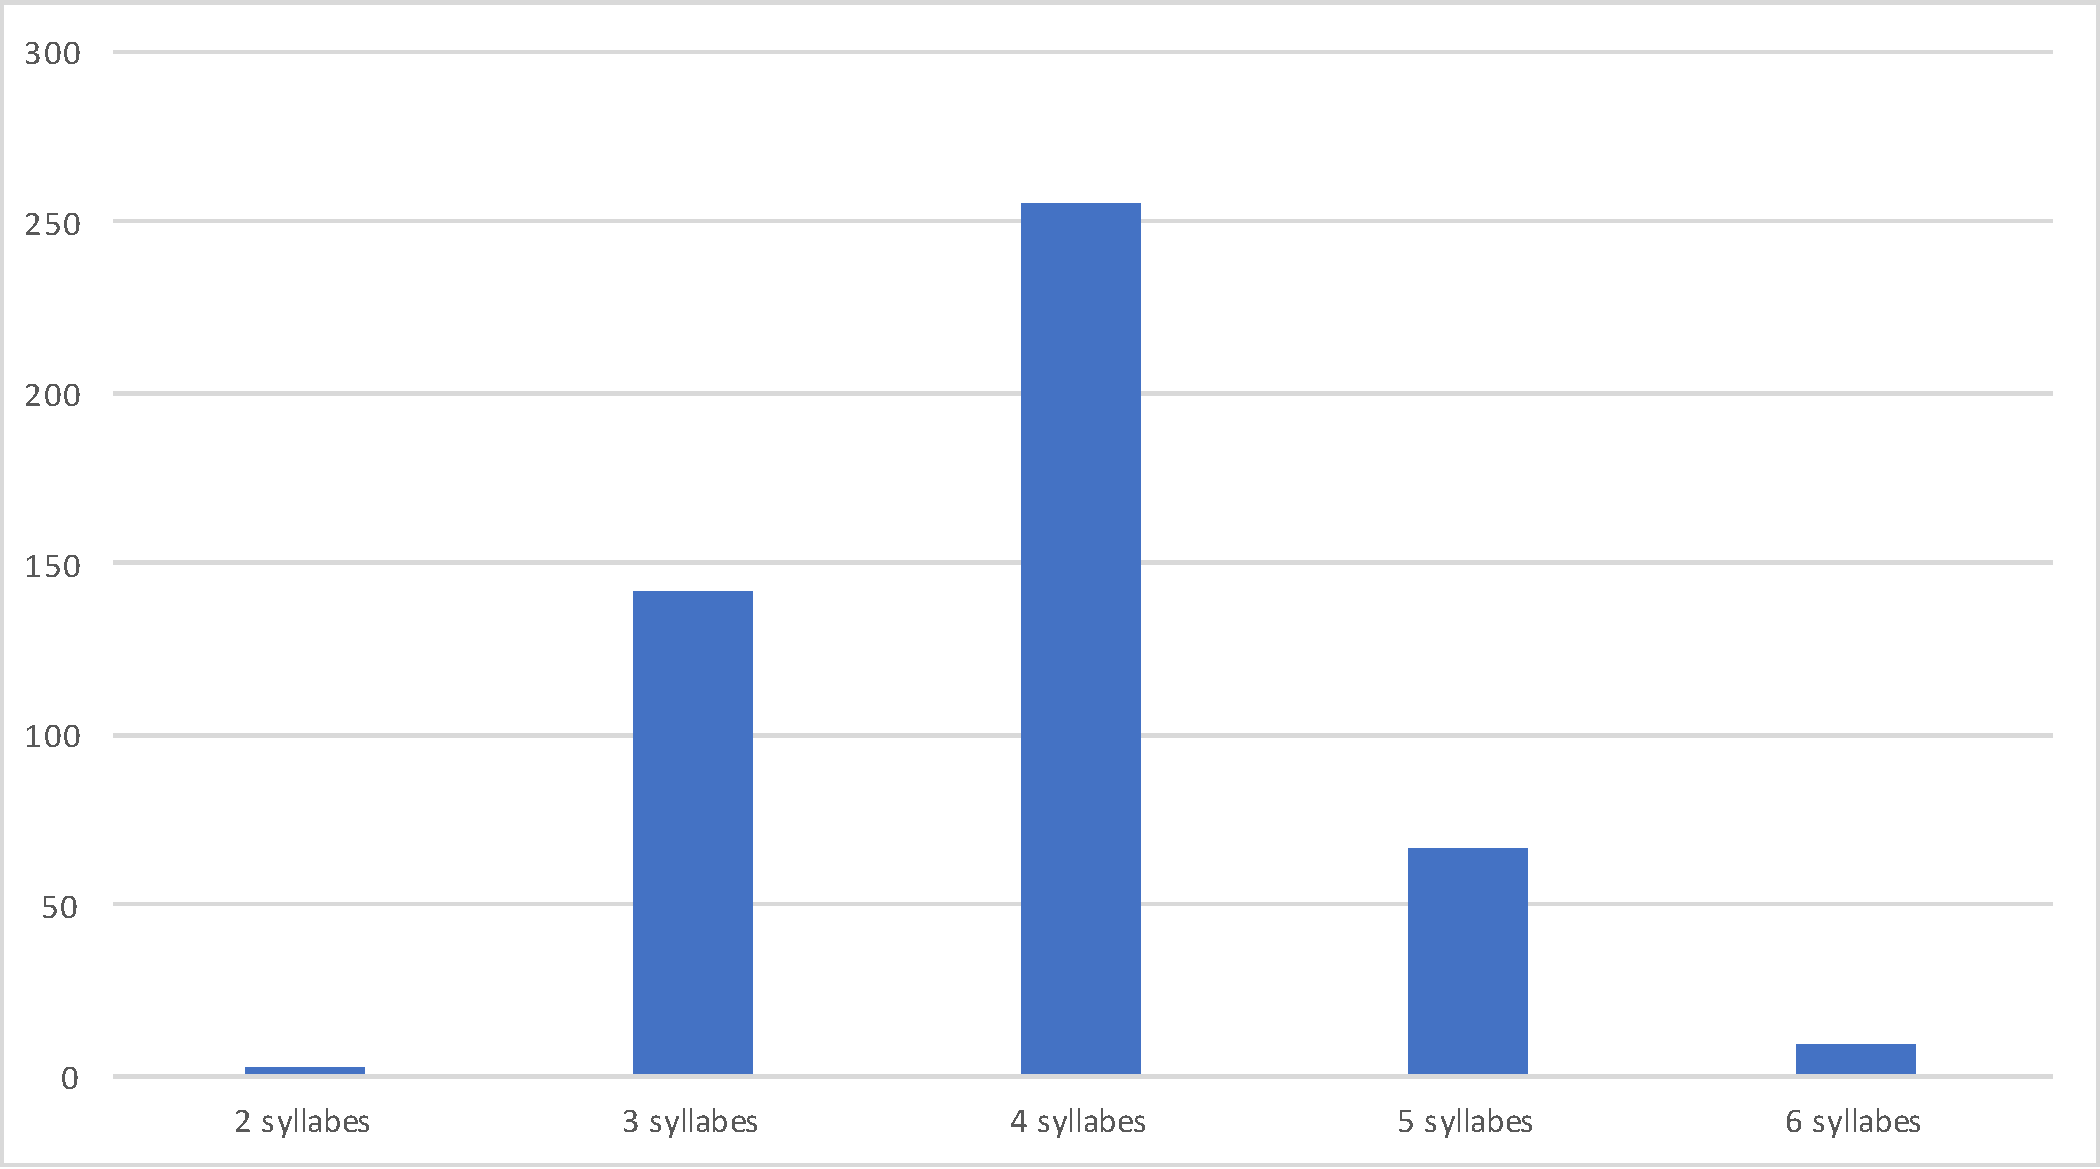
\includegraphics[height=.3\textheight]{figures/montermini-1-crop.pdf}}
\caption{Distribution des lexèmes en \textsc{-phone} selon le
nombre de syllabes}
\label{fig:Montermini:1}
\end{figure}

Le fonctionnement de la contrainte de taille\is{constraint!size constraint} montre que, contrairement à
ce que l'on aurait pu imaginer, le poids de \emph{francophone} en tant
que \isi{leader word} de la série est limité, du moins en ce qui concerne la
taille\is{constraint!size constraint} des dérivés. En effet, on aurait pu s'attendre à ce que le format
trisyllabique prévale, éventuellement au prix de la réduction de bases\is{base}
trop longues. Cependant, si on regarde les lexèmes en \textsc{-phone}
les plus fréquents dans FrWac, \emph{francophone} vient, sans surprise,
largement en tête, mais les dix premiers se répartissent de manière
pratiquement équivalente entre tri- et quadrisyllabiques\footnote{Les
  dix lexèmes en question sont~: \emph{francophone}, \emph{anglophone},
  \emph{germanophone}, \emph{arabophone}, \emph{hispanophone},
  \emph{lusophone}, \emph{néerlandophone}, \emph{turcophone},
  \emph{berbérophone}, \emph{russophone}.}.

Parmi les 66 dérivés présents dans la base qui comportent cinq syllabes,
28 comportent également au moins une variante quadrisyllabique, la
plupart du temps obtenue par troncation du thème\is{stem} de base\is{base} (type (5g), par
exemple \emph{arménianophone} / \emph{arménophone}, \emph{tibétanophone}
/ \emph{tibétophone}). Il en va de même pour 4 des 9 dérivés qui
comportent 6 syllabes (\emph{américanophone} / \emph{américophone}).
Inversement, sur 23 dérivés qui ont un radical\is{stem} obtenu par troncation de
la base\is{base}, 22 possèdent une variante «~longue~», généralement comportant une
syllabe de plus. De la même manière, sur 91 lexèmes relevant du type
(5e) (emploi du même thème\is{stem} que celui d'un gentilé), 79 comportent trois
ou quatre syllabes. Nous pouvons donc considérer que le format tri- ou
quadrisyllabique permet de satisfaire une contrainte de taille\is{constraint!size constraint} qui veut
que, dans un mot construit, la base\is{base} corresponde le plus fréquemment au
format dissyllabique %
%(cf. Plénat 2009)
\citep[cf.][]{Plenat09}%
%Plénat
%
~; les troncations de thème\is{stem} ont
principalement pour but de satisfaire cette contrainte\is{constraint} (au détriment,
bien entendu, de la contrainte de fidélité\is{constraint!faithfulness constraint} base-dérivé).

Concernant les propriétés segmentales des dérivés en correspondance de
l'exposant, 79,5\% des cas (378) se terminent en {[}ɔfɔn{]} et 20,5\%
(97) se terminent en {[}fɔn{]} précédé d'un autre segment (la plupart du
temps une voyelle, cf. ci-dessous). À ce propos, il est possible
d'établir une corrélation intéressante~: pour le second groupe, le
segment qui précède {[}fɔn{]} est déjà présent dans le thème\is{stem} de base\is{base}
dans la totalité des cas, alors que pour le premier groupe, celui se
terminant en {[}ɔfɔn{]}, le thème\is{stem} de base\is{base} ne comporte un {[}o{]} final
que dans 40 dérivés sur 378, répartis comme suit~:

\ea\label{ex:montermini:6}

  \ea thèmes\is{stem} se terminant en {[}o{]} (\emph{espérantophone},
\emph{lesothophone}) 17

  \ex thèmes\is{stem} tronqués en correspondance d'un {[}o{]} (\emph{lettophone},
\emph{tagalophone}) 10

  \ex thèmes\is{stem} supplétifs savants\is{stem!learned}\footnote{Je considère que les thèmes\is{stem}
  supplétifs savants\is{stem!learned} comportent un {[}o{]} final, dans la mesure où ils
  peuvent apparaître sous cette forme, par exemple dans des composés\is{compounding}
  (\emph{germano-soviétique}, \emph{sino-japonais}).}
(\emph{germanophone}, \emph{sinophone}) 13
\z\z

La figure \ref{fig:Montermini:2} résume la situation décrite («~oui~» indique que le segment
précédant {[}fɔn{]} est présent dans le thème\is{stem} de base\is{base}, «~non~» qu'il ne
l'est pas).

\begin{figure} 
{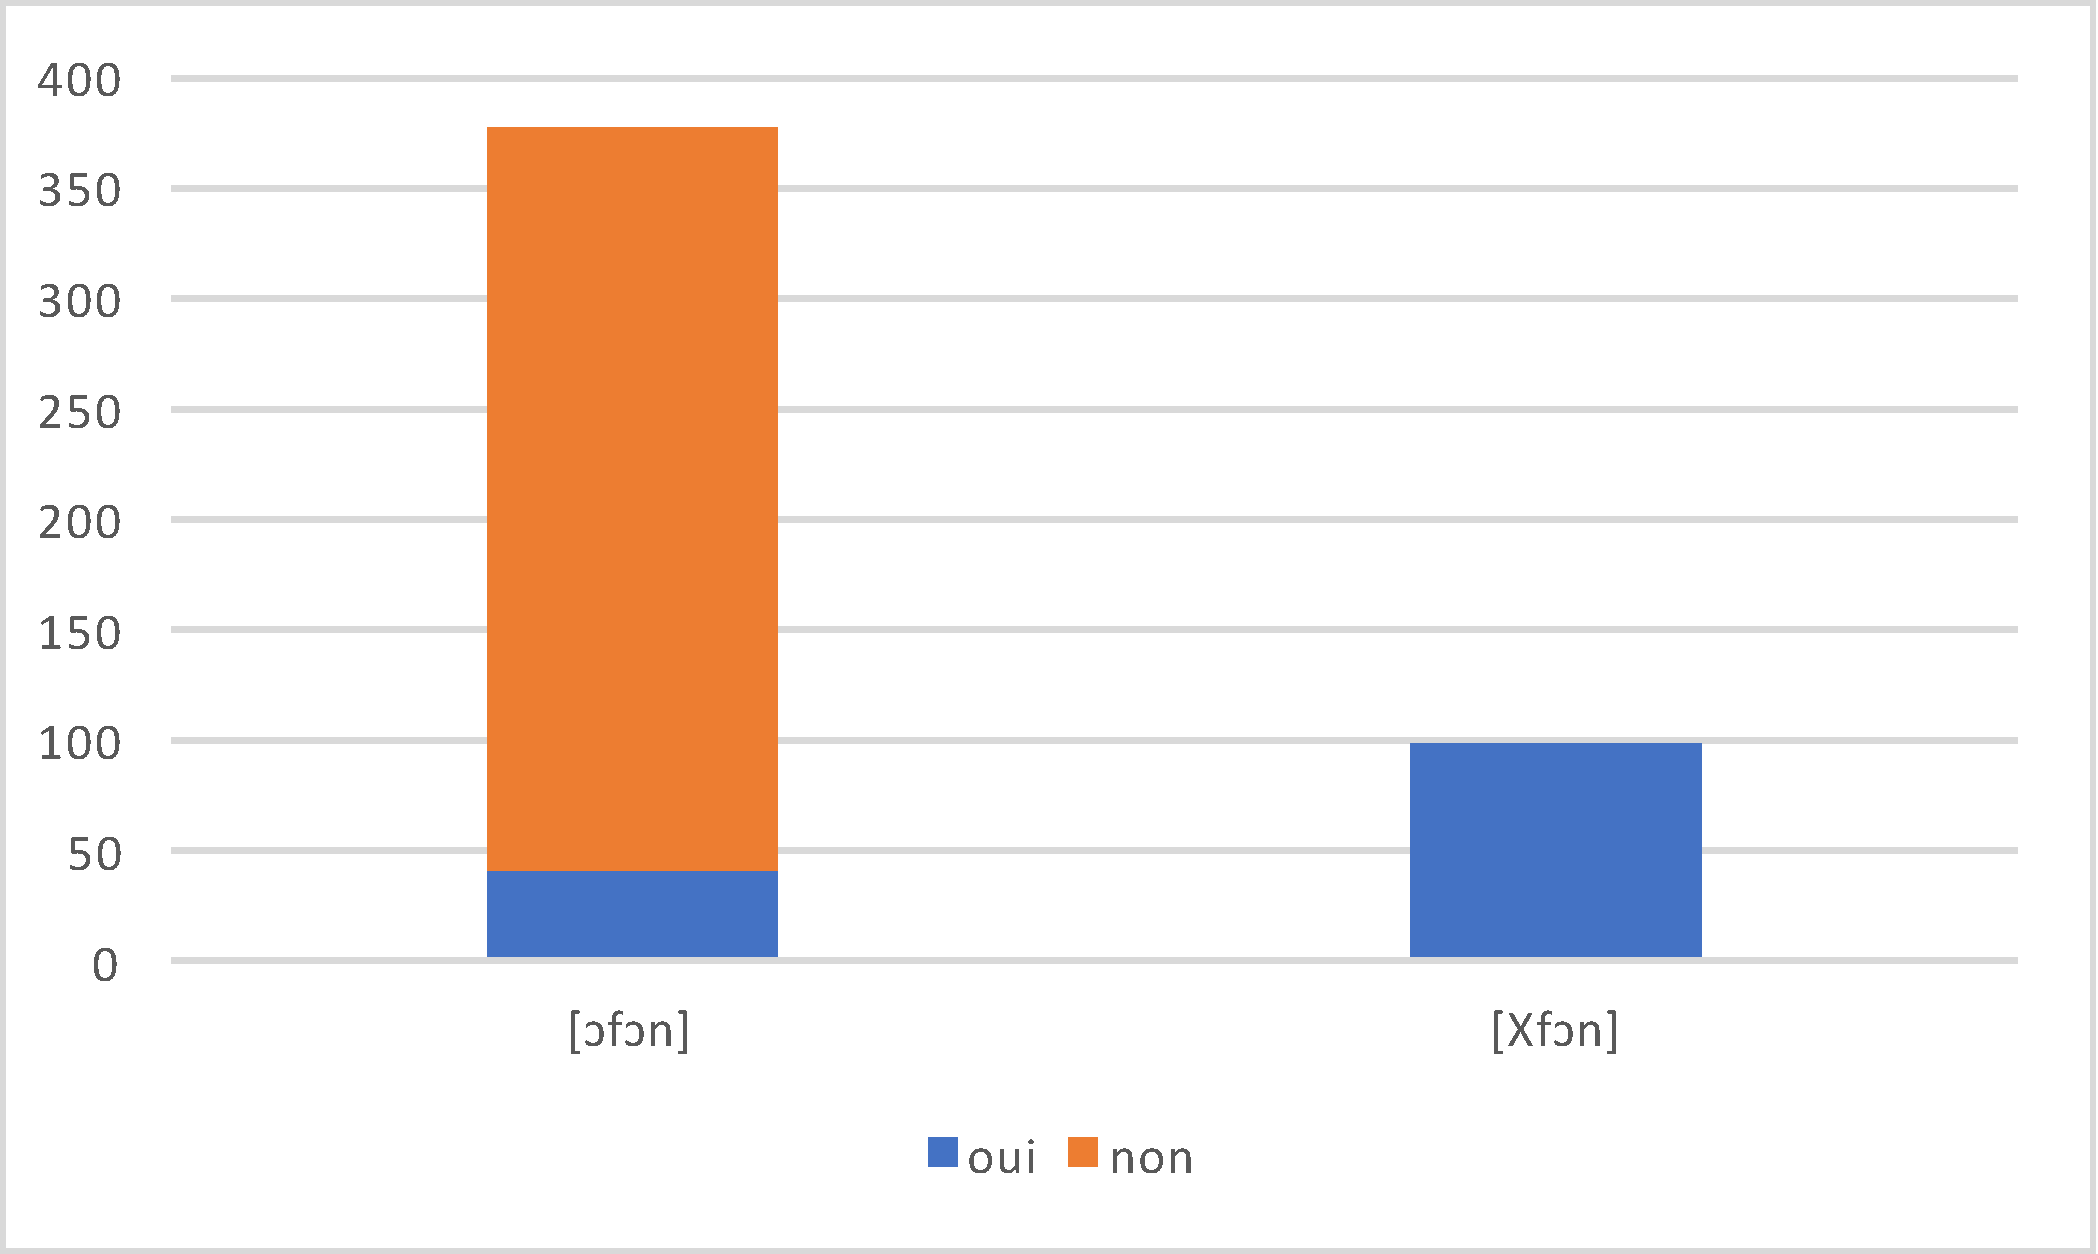
\includegraphics[height=.3\textheight]{figures/montermini-2-crop.pdf}}
\caption{Distribution des segments précédant {[}fɔn{]}
présents ou non présents dans la base}
\label{fig:Montermini:2}
\end{figure}

Pour 338 lexèmes de la base de données (71,2\% du total), donc,
l'opération phonologique consiste simplement en la concaténation de la
séquence {[}ɔfɔn{]} à un thème\is{stem}, modifié ou pas~; pour 30 autres (les cas
(6a) et (6c) ci-dessus), nous pouvons considérer que la présence d'un
{[}o{]} dans la base\is{base} n'est rien de plus que fortuite. Seuls les 10
lexèmes du type (6b) manifestent une manipulation dont l'effet est
d'avoir un thème\is{stem} se terminant par {[}o{]}~; cependant, dans ce cas, la
réduction du thème\is{stem} a aussi pour effet de produire un dérivé tri- ou
quadrisyllabique dans la totalité des cas. On peut donc considérer
qu'ici, au mieux, on assiste à une convergence entre la contrainte de
taille\is{constraint!size constraint} et la contrainte\is{constraint} qui demande que le dérivé se termine en
{[}ɔfɔn{]}.

Considérons maintenant les 97 cas dans lesquels le dérivé ne se termine
pas par {[}ɔfɔn{]}. Tout d'abord, plus de deux tiers de ces dérivés (66)
possèdent également une variante en {[}ɔfɔn{]}. De plus, comme je l'ai
observé, il s'agit toujours de cas comme ceux exemplifiés en (7), dans
lesquels le segment qui précède {[}fɔn{]} est toujours déjà présent dans
le thème\is{stem} de base\is{base} en tant que segment final. En (7) je donne le détail du
nombre de dérivés selon la séquence finale~:

\ea\label{ex:montermini:7}
    \ea {[}afɔn{]} \emph{aymaraphone} 34

    \ex {[}ifɔn{]} \emph{swahiliphone} 28

    \ex {[}efɔn{]} \emph{malinképhone} 9

    \ex {[}Cfɔn{]} \emph{tamoulphone} 8

    \ex {[}wafɔn{]} \emph{danoiphone} 6

    \ex {[}ãfɔn{]} \emph{flamanphone} 5

    \ex {[}ufɔn{]} \emph{ourdouphone} 4

    \ex {[}œfɔn{]} \emph{banlieuphone} 3
\z\z

On pourrait être tenté d'identifier les formes {[}afɔn{]} et {[}ifɔn{]}
comme des sous-défauts, vu leur prépondérance dans cette classe de
dérivés. Il est probable, cependant, que leur fréquence soit surtout
liée à la fréquence globale des noms de langues se terminant par {[}a{]}
ou {[}i{]} par rapport aux autres segments. Notons que les 89 dérivés
dans lesquels {[}fɔn{]} est précédé d'une voyelle différente de {[}o{]}
constituent la majorité des outputs pour les thèmes\is{stem} de base\is{base} se terminant
en voyelle. La base de données comprend en effet 58 autres dérivés de
bases\is{base} en voyelles, dans lesquels soit la voyelle est effacée en faveur
de {[}ɔfɔn{]} (\emph{bambarophone}), soit, bien plus rarement
(uniquement 6 exemples), la séquence {[}ɔfɔn{]} est attachée après la
voyelle (presque uniquement un {[}i{]}, \emph{thaïophone}) (notons, de
plus, que dans ce cas il s'agit toujours de bases\is{base} brèves, susceptibles
de donner des dérivés tri- ou quadrisyllabiques).

Une interprétation des données présentées consiste à attribuer à la
construction en question une forme d'exposant par défaut qui est
{[}ɔfɔn{]}, et une variante hiérarchiquement subordonnée, {[}Vfɔn{]} (où
V représente une voyelle quelconque). L'ensemble des contraintes\is{constraint}
formelles (de série) qui pèsent sur les outputs de cette construction
stipule donc qu'un dérivé doit comporter quatre (à défaut trois)
syllabes et se terminer en {[}ɔfɔn{]} (à défaut en {[}Vfɔn{]}). Le reste
des propriétés formelles observées pour les dérivés en question provient
des autres contraintes\is{constraint} générales qui pèsent sur la forme des mots
construits, et en particulier de la contrainte de fidélité\is{constraint!faithfulness constraint} base-dérivé,
qui est responsable de la forme des lexèmes en (7) et, plus en général
du timbre de la voyelle qui précède {[}fɔn{]} lorsque ce n'est pas un
{[}o{]}. À son tour, la contrainte de fidélité\is{constraint!faithfulness constraint} interagit avec les autres
contraintes\is{constraint} qui sont responsables pour la sélection et/ou la
modification des thèmes\is{stem} de base\is{base}, par exemple la contrainte de famille\is{constraint!family}.
Si une base\is{base} est isolée dans sa famille lexicale (c'est le cas de la
majorité des noms de langues non européennes), alors la sélection du
thème\is{stem} n'est pas un enjeu~: c'est le thème\is{stem} unique qui est choisi et qui
est éventuellement manipulé pour satisfaire d'autres contraintes\is{constraint}. Au
contraire, si la base\is{base} appartient à une famille lexicale nombreuse, le
thème\is{stem} sélectionné peut correspondre au nom de la langue, construit ou
pas %
%(\emph{coréanophone}, \emph{corsophone}, \emph{picardophone}, cela
%correspond, grosso modo à la «~Contrainte de fidélité à la forme libre~»
%de Roché \& Plénat 2014~: 1873)
\citep[\emph{coréanophone}, \emph{corsophone}, \emph{picardophone}, cela correspond, grosso modo, à la «~Contrainte de fidélité à la forme libre~» de][1873]{Roche14}%
%Roché-Plénat
%
, à un thème\is{stem} supplétif savant\is{stem!learned}
(\emph{francophone}, \emph{lusophone}, \emph{magyarophone}), ou bien,
moins préférentiellement, au thème\is{stem} qui apparaît devant les affixes
construisant des gentilés et qui correspond, dans la plupart des cas,
comme je l'ai observé, à un nom géographique de pays, région, etc.
(\emph{islandophone}, \emph{japonophone}). Concernant ce dernier cas, la
plupart des dérivés sont ambigus, comme ceux mentionnés~; cependant, il
est possible que, du moins pour certains locuteurs, les deux
possibilités soient disponibles. Dans certains cas, en effet, le thème\is{stem}
de base\is{base} correspond sans ambiguïté soit au thème\is{stem} qui précède un suffixe
ethnique (\emph{champenophone}, \emph{néerlandophone}) soit à un nom
géographique (\emph{allemagnophone}, \emph{portugalophone}). Ainsi, s'il
existe un nom en \protect\hypertarget{OLEux5fLINK1}{}{}\textsc{-phone}
construit sur une base\is{base} supplétive savante\is{stem!learned}, qu'elle soit ambiguë (8a) ou
pas (8b-c) par rapport à un autre thème\is{stem}, on peut rencontrer des
variantes qui font prévaloir la fidélité à la forme libre du nom de la
langue (souvent homophone à un ethnique) et/ou d'un nom de pays~:

\ea\label{ex:montermini:8}
\begin{tabular}[t]{@{}lll}
a. & {italophone} & {italianophone}\\
b. & {germanophone} & {allemandophone}, {allemagnophone}\\
c. & {hispanophone} & {espagnolophone}, {espagnophone}\\
\end{tabular}
\z

Considérons maintenant les données de l'italien. Le premier fait à
remarquer est que tous les lexèmes présents dans le corpus comportent,
avant la séquence {[}fon{]}, un {[}o{]} qui porte l'accent tonique de
mot, et ont donc la structure {[}Xˈɔfono{]}\footnote{La hauteur des
  voyelles moyennes n'est pas importante dans ce contexte, puisqu'elle
  est phonologiquement déterminée par la place de l'accent. Pour avoir
  une représentation phonologique complète, j'indique la forme du
  masculin singulier (finale en \emph{-o}), mais ce qui suit s'applique
  à toutes les formes fléchies des lexèmes en \textsc{-fono} (finales en
  -\emph{a}, -\emph{i}, -\emph{e}).}. L'exposant possède donc une forme
fixe à la fois plus contrainte\is{constraint} et plus longue qu'en français. Puisque,
je le rappelle, je considère qu'un exposant est simplement une séquence
phonologique associée de façon arbitraire à une construction, on ne doit
pas nécessairement chercher des raisons qui expliquent la plus grande
rigidité de l'italien par rapport au français dans la forme de celui-ci.
Il est possible, néanmoins, qu'une des raisons réside dans le fait que
l'italien tolère moins bien une variation sur une voyelle qui porte
l'accent primaire de mot, même si l'on peut remarquer que cette voyelle
n'est pas toujours {[}ɔ{]} lorsque le dérivé n'est pas un nom de
locuteurs (\emph{telèfono}, \emph{vibràfono}).

Du point de vue prosodique, on observe une plus grande dispersion des
formats possibles, avec une prédominance du format pentasyllabique, mais
avec presque autant de lexèmes à quatre ou à six syllabes, comme le montre la figure \ref{fig:Montermini:3}.

\begin{figure} 
{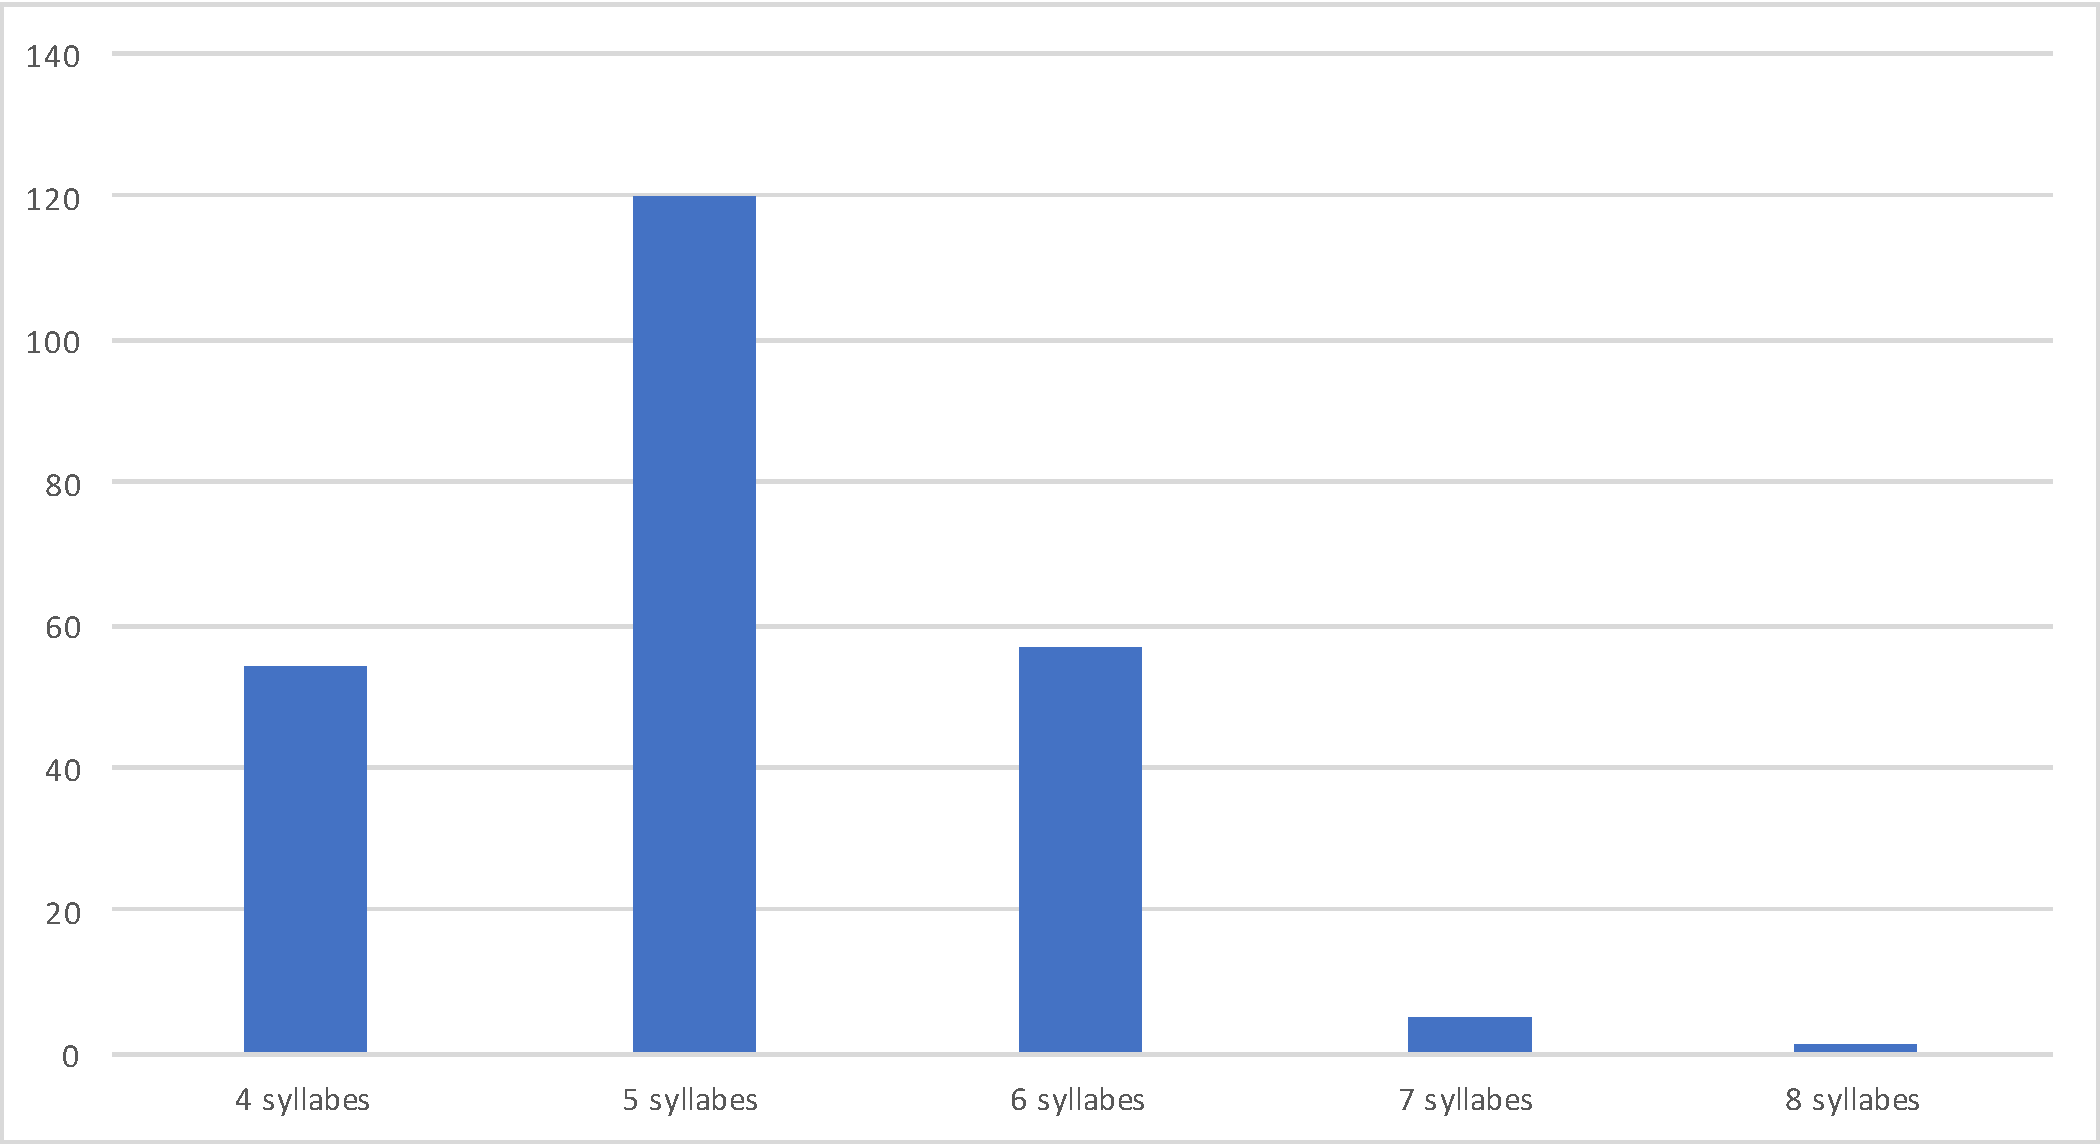
\includegraphics[height=.3\textheight]{figures/montermini-3-crop.pdf}}
\caption{Distribution des lexèmes en \textsc{-fono} selon le
nombre de syllabes}
\label{fig:Montermini:3}
\end{figure}

Comme il a déjà été observé dans d'autres cas, la contrainte de taille\is{constraint!size constraint}
est donc moins forte en italien qu'en français, et elle est certainement
soumise à la contrainte de fidélité\is{constraint!faithfulness constraint} base-dérivé. Concernant
l'interaction entre la base\is{base} et l'exposant, le cas par défaut en italien
est celui dans lequel la séquence {[}ɔfono{]} est directement accolée au
thème\is{stem} de base\is{base}, si celui-ci se termine en consonne (\emph{amazighofono},
\emph{yiddishofono}), ou bien -- plus fréquemment -- la voyelle finale
de la base\is{base} est effacée (\emph{bantofono}, \emph{ligurofono},
\emph{quechuofono}). À eux seuls, ces cas couvrent exactement deux tiers
des dérivés de la base (158 sur 237), auxquels nous pouvons rajouter 22
cas dans lesquels la base\is{base} est un thème\is{stem} supplétif d'origine savante\is{stem!learned}.
75,9\% des dérivés ne posent donc aucun problème particulier, ni pour le
choix du thème\is{stem} de base\is{base}, ni pour l'interaction phonologique entre ce
thème\is{stem} et l'exposant. Concernant le phénomène d'effacement de la voyelle
finale en dérivation en italien\footnote{Cf. %
%Montermini (2010) 
\citet{Montermini10} %
%Montermini
%
pour une
  discussion.}, deux hypothèses sont possibles, dans un cadre de
morphologie thématique\is{morphology!stem spaces framework} basée sur les contraintes\is{constraint}~: i) le thème\is{stem}
sélectionné est un thème\is{stem} dépourvu de voyelle, le même que l'on retrouve
dans d'autres dérivés, qui est sélectionné en respectant la contrainte
de famille~; ii) le thème\is{stem} sélectionné est un thème\is{stem} qui contient une
voyelle (par exemple un thème\is{stem} qui coïncide formellement avec une des
formes fléchies), qui est effacée sous l'effet d'autres contraintes\is{constraint}, par
exemple une contrainte phonologique anti-hiatus. Les deux hypothèses en
question ne sont pas nécessairement inconciliables. La première peut
être valable pour les bases\is{base} qui appartiennent à des familles lexicales
nombreuses, alors que pour les autres il est plus difficile d'imaginer
qu'un thème\is{stem} sans voyelle soit déjà présent dans le lexique. De plus,
comme j'ai essayé de le montrer dans des travaux précédents %
%(Montermini 2003, 2010)
\citep{Montermini2003,Montermini10}%
%
, l'effacement de voyelle en dérivation est un phénomène qui,
au moins en partie, est aussi influencé par la phonologie, avec des
voyelles qui sont plus facilement effaçables que d'autres. 
\largerpage
Dans la base
de données considérée ici on retrouve en effet deux exemples de
non-effacement de voyelle, \emph{bantuofono} et \emph{urduofono} (qui
coexistent avec les formes plus «~régulières~» \emph{bantofono} et
\emph{urdofono}). Le fait que dans les deux cas la voyelle non effacée
est un {[}u{]} n'est peut-être pas un hasard, puisqu'il s'agit de la
voyelle qui en général résiste plus à l'effacement en italien (cf. les
travaux cités ci-dessus).

En ce qui concerne le petit quart de dérivés restants, la quasi-totalité
présentent des réductions du thème\is{stem} et peuvent être répartis en deux
groupes. Les deux contiennent majoritairement des lexèmes qui sont des
variantes d'autres lexèmes construits plus «~régulièrement~». Le premier
groupe, plus nombreux (45 lexèmes), correspond au cas déjà relevé pour
le français dans lequel un lexème en -\textsc{fono} est construit à
partir d'un thème\is{stem} qui sert aussi de base\is{base} à des gentilés et/ou à un nom
géographique. Comme en français, on y retrouve de nombreux cas dans
lesquels le thème\is{stem} de la base\is{base} est ambigu de ce point de vue (\ref{ex:montermini:9a}), ainsi
que des cas, plus rares, dans lesquels le thème\is{stem} est sans ambiguïté soit
un thème\is{stem} de gentilés (\ref{ex:montermini:9b}), soit un nom géographique (\ref{ex:montermini:9c})~:

\ea\label{ex:montermini:9}

\ea\label{ex:montermini:9a}  {islandofono}, {milanofono}

\ex\label{ex:montermini:9b}   {portogofono}

\ex\label{ex:montermini:9c}   {polonofono}
\z\z

Le deuxième groupe, plus restreint (5 lexèmes au total), comprend des
dérivés dans lesquels le thème\is{stem} est réduit au format bisyllabique,
indépendamment de sa structure morphologique (\emph{albofono},
\emph{estofono}, \emph{lettofono}). Cette tendance, marginale, à avoir
des bases\is{base} bisyllabiques (et donc des dérivés quadrisyllabiques) doit
très probablement être attribuée à la tendance que présentent les
éléments de composition\is{compounding!neoclassical} d'origine néoclassique, surtout initiaux, à être
bisyllabiques en italien %
%(cf. Thornton 2007~: 253-259)
\citep[cf.][253--259]{Thornton2007}%
%Thornton
%
. Il est possible
que, pour certains locuteurs, un nom en -\textsc{fono} doive encore se
conformer au format d'un composé\is{compounding!neoclassical} néoclassique (peut-être sur l'exemple
des dérivés dans lesquels la base\is{base} est un thème savant\is{stem!learned}). Cependant, vu le
nombre de lexèmes concernés, il s'agit d'une tendance minoritaire, voire
résiduelle, ce qui peut être considéré comme une preuve indirecte du
fait qu'en synchronie ces formations tendent à être manipulées par les
locuteurs comme des dérivés affixaux à part entière. À la différence du
français, il est difficile d'établir une corrélation précise entre ces
réductions du thème\is{stem} de base\is{base} et une quelconque contrainte prosodique,
puisque, comme nous l'avons vu, les contraintes\is{constraint} de taille\is{constraint!size constraint} sont moins
importantes en italien, et probablement subordonnées aux contraintes\is{constraint} de
fidélité\is{constraint!faithfulness constraint}.

Pour conclure sur l'analyse de l'italien, les deux contraintes\is{constraint} qui
semblent prévaloir dans la construction des noms en -\textsc{fono} sont
la contrainte\is{constraint} sur la forme des dérivés, qui unit, en réalité, plusieurs
contraintes\is{constraint} segmentales et prosodiques, et qui stipule qu'ils doivent
avoir la structure {[}Xˈɔfono{]}, sans contrainte\is{constraint} forte sur le nombre de
syllabes, et la contrainte de fidélité\is{constraint!faithfulness constraint} base-dérivé. Ceci entraîne une
tendance moins grande qu'en français à modifier les thèmes\is{stem} des bases\is{base}
pour satisfaire des contraintes\is{constraint} prosodiques ou segmentales.

Ce que la comparaison entre les deux langues montre est que des
constructions apparemment similaires, dans le processus de leur
intégration aux systèmes phonologiques et morphologiques des langues en
question, peuvent en réalité se développer comme des jeux de contraintes\is{constraint}
agencées de manière différente. L'italien a développé une construction
dans laquelle la forme de l'exposant est fortement contrainte\is{constraint} et la
fidélité\is{constraint!faithfulness constraint} entre la base\is{base} et le dérivé prime sur les autres contraintes\is{constraint}
formelles, alors que les contraintes\is{constraint} prosodiques de taille\is{constraint!size constraint} ont moins de
poids. En français, en revanche, ces contraintes\is{constraint} jouent un rôle
important, comme dans les autres procédés affixaux, ce qui, combiné à la
contrainte de fidélité\is{constraint!faithfulness constraint} base-dérivé, entraîne une diversification des
structures segmentales possibles pour l'exposant, qui, s'il contient
toujours de préférence une voyelle étymologique de timbre /o/ à la
jonction entre le thème\is{stem} de la base\is{base} et l'exposant, admet d'autres
voyelles, voire d'autres segments dans la même position.

\subsection{-\textsc{issimo} et -\textsc{issime}}

La deuxième étude de cas concerne un suffixe du français qui n'a pas
encore suscité, à ma connaissance, l'intérêt des linguistes et des
lexicographes. Il s'agit du suffixe -\textsc{issimo}, que l'on retrouve
notamment dans la construction de noms d'enseignes, événements, marques
ou produits, les plus connus étant probablement \emph{Colissimo} et
\emph{Doctissimo}\footnote{L'ensemble des lexèmes en -\textsc{issimo}
  cités dans cette section est donné en Annexe, avec une indication de
  leur signification dans les contextes dans lesquels ils ont été
  repérés.}. Cependant, on peut également repérer des contextes dans
lesquels des lexèmes en ‑\textsc{issimo} sont créés et employés en
discours par les locuteurs, comme les suivants\footnote{Il est possible
  que pour ces emplois de lexèmes en -\textsc{issimo} en discours les
  contraintes\is{constraint} catégorielles et sémantiques pèsent plus lourd que les
  contraintes\is{constraint!formal} formelles par rapport à ceux qui servent de dénominations
  commerciales, en les rendant, de ce point de vue, plus proches des
  lexèmes en -\textsc{issime} (et des autres lexèmes construits
  «~canoniques~»). Cependant, j'ai recensé trop peu d'exemples de ce type
  pour pouvoir tirer des conclusions fiables. Si cela est vrai,
  l'ordonnancement des contraintes\is{constraint} serait également influencé par des
  paramètres externes à la morphologie liés à l'emploi pragmatique et
  sociolinguistique des lexèmes construits. (Je remercie le relecteur de
  cet article pour m'avoir fait réfléchir sur ce point).}~:

  \ea\label{ex:montermini:10}

  \ea\label{ex:montermini:10a}
Enfin bref je suis tout le contraire de ce qu'il aime c'est ça le plus
drolissimo.

{[}Twitter, 4 novembre 2013{]}

\ex\label{ex:montermini:10b}
J'ai un «~torticolissimo~». C'est-à-dire que mon cou est coincé depuis 3
semaines et que personne ne sait quand la situation sera débloquée.

{[}Twitter, 26 mai 2015{]}

\ex\label{ex:montermini:10c} C'était vraiment énorme ! L'entrée de Médine énorme. Daniel Allouche
(speaker), énorme. Le public havrais, énormissimo (sic).
[\url{http://www.lebannerofficial.com/index.php?option=com_content&task=view&id=355}]
\z\z

Les lexèmes ci-dessus occupent une position canonique de noms ou
adjectifs, et véhiculent un sens génériquement appréciatif / superlatif.
En ce sens, le suffixe en question est proche du suffixe
-\textsc{issime}, qui a la même origine, mais une histoire différente.
Les deux sont issus du suffixe latin superlatif -\emph{issimus}. Selon
les dictionnaires, -\textsc{issime} est rentré en français via l'italien
à partir du XIV\textsuperscript{e} siècle, d'abord via des mots
d'adresse comme \emph{sérénissime} %
%(Perko 2010)
\citep{Perko2010}%
%Perko
%
. En ce qui concerne
-\textsc{issimo}, son origine italienne est rendue encore plus évidente
par la voyelle {[}o{]} finale (on peut d'ailleurs considérer qu'il
possède une variante en {[}a{]}, par exemple dans \emph{Diorissima},
\emph{Naturissima}, etc.). Sans en avoir la certitude, je présume que sa
disponibilité en français a été renforcée par l'existence d'un certain
nombre de mots du vocabulaire musical directement empruntés à l'italien
(\emph{fortissimo}, \emph{pianissimo}, etc.). Les premières attestations
que j'ai pu documenter remontent à la seconde moitié des années 1960~:
\emph{Vernissimo} apparaît dans le slogan d'une annonce de vernis pour
ongles de 1966, \emph{Parfumissimo} dans une annonce de savons de 1969
et \emph{Erotissimo} est le titre d'un film de 1969. Comme je l'ai
montré ci-dessus, le suffixe, d'abord employé dans des dénominations, a
partiellement pénétré dans la langue courante. Il est intéressant de
remarquer que, si parfois il est employé dans des contextes spécifiques
à la réalité italienne (ou plus généralement «~latine~»), ceci n'est
absolument pas systématique, comme le montre en particulier la troisième
attestation de (\ref{ex:montermini:10}).

Pour cette étude, j'ai rassemblé une base de données de 294 lexèmes.
Comme dans le cas des -\textsc{phone}, la base a été recueillie en
rassemblant en premier lieu les mots se terminant par les séquences
\textless{}issimo\textgreater{} ou \textless{}issima\textgreater{} dans
FrWac. Ici aussi, la liste a été nettoyée manuellement~; de plus, le
contexte de chaque forme a été vérifié afin d'éliminer les nombreux
exemples provenant de pages écrites en italien ou en latin ramassées par
FrWac. Également, tous les mots du vocabulaire musical auxquels j'ai
fait allusion ci-dessus, ainsi que d'autres qui étaient clairement des
emprunts directs (par exemple \emph{campionissimo}) ont été éliminés.
Pour terminer, la liste a été complétée par des mots en -\textsc{issimo}
provenant de différentes sources\footnote{Une liste contenant de
  nombreux mots en -\textsc{issimo} m'a été fournie par ma collègue
  Antonella Capra, que je remercie.}, et par des recherches ciblées sur
le Web. Parallèlement, j'ai rassemblé une liste de 373 lexèmes en
-\textsc{issime} présents dans FrWac, que je compare à ceux en
-\textsc{issimo}.

Concernant tout d'abord ce dernier suffixe, il s'attache principalement
à des adjectifs ou des noms pour former des superlatifs\footnote{Dans
  toute la base on ne trouve qu'un seul lexème en -\textsc{issime} qui
  est indubitablement construit sur un mot qui n'est ni un nom ni un
  adjectif~: \emph{obligatoirementissime}.}. Du point de vue formel,
%
%Plénat (2002) 
\citet{Plenat2002a} %
%Plénat
%
a identifié au moins quatre paramètres pour définir son
comportement~:

\begin{enumerate}[label=\roman*)]
\item il s'agit d'un suffixe «~mi-savant~», qui peut sélectionner tant des
thèmes savants\is{stem!learned} que des thèmes\is{stem} populaires (\emph{universalissime} vs.
\emph{naturellissime})~;

\item le suffixe -\emph{ique} peut être effacé devant -\textsc{issime}
(\emph{catholissime}, \emph{nostalgissime})~;

\item la rime (voyelle et consonne finales) tombe si le thème\is{stem} de base\is{base} est
tri- ou quadrisyllabique et se termine par une consonne sifflante
latente\is{latent consonant} (\emph{bruxellissime}, \emph{rigourissime})~;

\item la rime tombe si le thème\is{stem} de base est tri- ou quadrisyllabique et
se termine par un {[}i{]} suivi d'une consonne latente\is{latent consonant}
(\emph{favorissime}, \emph{interdissime}).
\end{enumerate}

Les propriétés i) et ii) captent plutôt des tendances que des règles. La
deuxième en particulier connaît plusieurs exceptions
(\emph{critiquissime}, \emph{sympathiquissime}), pour lesquelles Plénat
fait l'hypothèse que les lexèmes en question ont sélectionné un thème\is{stem}
populaire, alors que ce sont les thèmes savants\is{stem!learned} qui perdent la séquence
{[}is{]} devant -\textsc{issime} pour respecter la contrainte de
dissimilation\is{constraint!dissimilation constraint} (\emph{catholissime} vs. *\emph{catholicissime}). Les
données de FrWac semblent indiquer, dans ce cas, que -\textsc{issime}
tend plutôt à sélectionner des bases\is{base} populaires~: sur 23 dérivés
construits sur des bases\is{base} qui possèdent un thème\is{stem} L distinct des thèmes\is{stem} A
et B, 17 utilisent le thème\is{stem} A ou B (\emph{lamentablissime},
\emph{sensuelissime}, \emph{supérieurissime}), et seulement 6 utilisent
le thème\is{stem} L (\emph{formidabilissime}, \emph{prétenciosissime}).
Concernant les deux paramètres iii) et iv), les données tirées de FrWac
potentiellement concernées sont extrêmement rares, mais semblent tout de
même confirmer les hypothèses formulées par Plénat. Dans l'ensemble de
la base de données, on retrouve seulement trois lexèmes dans lesquels
les tendances identifiées ne sont pas vérifiées~: \emph{andalousissime},
\emph{prétenciosissime} (iii) et \emph{favoritissime} (iv). On peut tout
de même observer que, si ces lexèmes ne respectent pas les contraintes\is{constraint}
phonologiques (dissimilatives\is{constraint!dissimilation constraint}) qui sont à l'origine des principes en
question, ils respectent entièrement la fidélité\is{constraint!faithfulness constraint} base-dérivé. Dans la
base, on retrouve également quatre lexèmes qui correspondent à des cas
de surapplication des règles ci-dessus, c'est-à-dire des effacements qui
ont eu lieu là où on ne les aurait pas attendus~: \emph{Barbérissime},
\emph{Optalissime} (iii), \emph{splendissime} et \emph{sublissime} (iv).
Les deux derniers sont déjà discutés par Plénat~; concernant les deux
premiers, il s'agit d'hapax construits, respectivement, sur le nom
propre \emph{Barbéris} et sur \emph{Optalis}, qui est le nom commercial
d'une série de produits financiers. À propos des cas d'effacement
discutés par Plénat, cependant, il est intéressant d'observer un autre
fait. L'effet des effacements en question est que le radical\is{stem} sur lequel
le dérivé en -\textsc{issime} est construit est presque toujours
identique à des thèmes\is{stem} de la famille dérivationnelle de la base\is{base}, qui
dans la plupart des cas correspondent au thème\is{stem} d'un lexème autonome. C'est
le cas des exemples \emph{bruxellissime} et \emph{nostalgissime}, et
également des dérivés \emph{prestigissime} et \emph{ténébrissime},
présents dans FrWac. Dans une perspective plus actuelle, les cas en
question pourraient probablement être expliqués en termes de sélection
de thème\is{stem} plutôt qu'en termes d'effacement. Notons tout de même, pour
terminer, qu'un effacement a certainement lieu dans plusieurs cas
lorsque la base\is{base} se termine par une voyelle, et notamment par {[}e{]}, cas
où, dans les données de la base (six concernées au total), il est
systématique (\emph{branchissime}, \emph{pavissime} ← \emph{pavé}).
Globalement, en tout cas, les modifications des thèmes\is{stem} des bases\is{base} restent
extrêmement rares dans la base de données. Au total, elles ne concernent
que 32 lexèmes (moins de 10\% de la base), distribués comme il suit~:
\largerpage

\ea \label{ex:Montermini:12}


        \ea \label{ex:Montermini:12a}effacement d'une rime voyelle + sifflante~: 5
(\emph{prestigissime})

      \ex \label{ex:Montermini:12b} effacement d'une rime {[}i{]} + consonne~: 4 (\emph{érudissime})

      \ex \label{ex:Montermini:12c} effacement du suffixe -\emph{ique~}: 4 (\emph{exotissime})

      \ex \label{ex:Montermini:12d} effacement d'une voyelle finale~: 14 (\emph{branchissime},
\emph{pourrissime})

      \ex \label{ex:Montermini:12e} épenthèse~: 5 (\emph{absolutissime}, \emph{merveilleutissime})
\z\z

Concernant la structure prosodique des dérivés présents dans la base, la
distribution est semblable à celle observée pour les dérivés italiens en
-\textsc{fono}, avec une prédominance du format quadrisyllabique, mais
avec une dispersion des dérivés entre les formats \mbox{tri-,} quadri- et
pentasyllabique. La distribution des dérivés de la base de données selon
le nombre des syllabes est résumée dans la figure \ref{fig:Montermini:4}.

\begin{figure} 
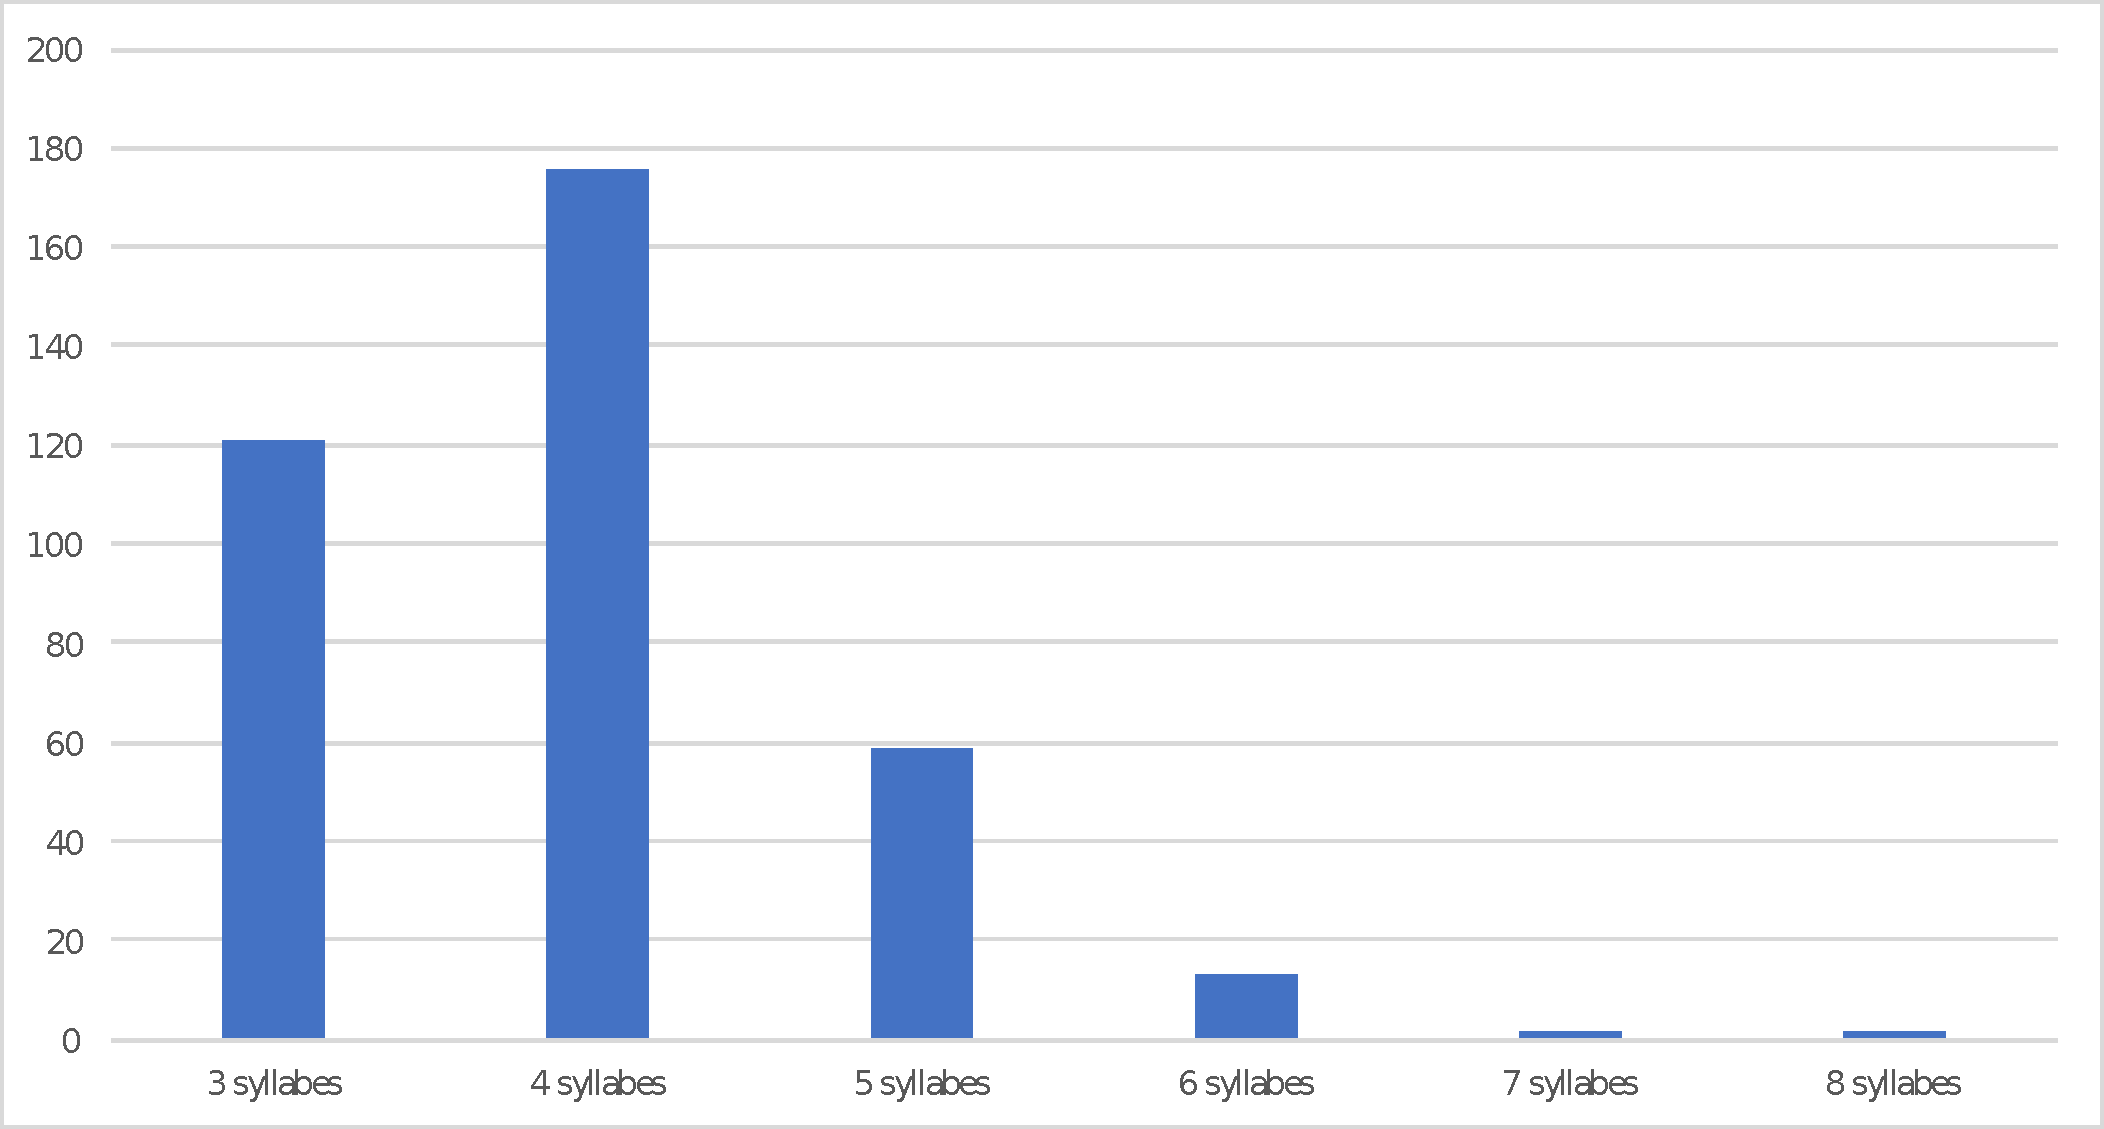
\includegraphics[height=.3\textheight]{figures/montermini-4.pdf}
\caption{Distribution des lexèmes en \textsc{-issime} selon le
nombre de syllabes}
\label{fig:Montermini:4}
\end{figure}


Une telle distribution peut être corrélée à la rareté des cas de
manipulation des thèmes\is{stem} de base\is{base} qui a été observée ci-dessus. La
concomitance entre ces deux facteurs semble en effet suggérer que les
contraintes\is{constraint} de taille\is{constraint!size constraint}, si elles sont actives, sont subordonnées à la
contrainte de fidélité\is{constraint!faithfulness constraint} base-dérivé~: la taille\is{constraint!size constraint} des dérivés dépend alors
plus de la taille des bases\is{base} (dont la longueur en syllabes est distribuée
de façon aléatoire) que de manipulations réalisées sur les thèmes\is{stem}.

Penchons-nous à présent sur les lexèmes en -\textsc{issimo}. La première
observation que nous pouvons formuler à leur égard concerne les
propriétés catégorielles et sémantiques du suffixe en question. Comme je
l'ai observé plus haut, à côté des cas «~canoniques~», comme ceux
exemplifiés en (\ref{ex:montermini:10}), -\textsc{issimo} sert souvent à construire des
dénominations d'enseignes commerciales, événements, marques, produits,
etc., ainsi que des occasionalismes destinés à être employés dans des
slogans. Sa valeur sémantique se limite donc dans la plupart des cas à
une valeur connotative superlative, voire génériquement positive. Les
bases\is{base} potentielles pour ce suffixe sont donc moins contraintes du point
de vue sémantique, et même catégoriel~; parfois, au contraire, la
sélection de la base (ou du thème\is{stem} de la base retenu) semble être faite
plutôt à partir de sa compatibilité formelle avec la construction que de
sa compatibilité sémantique. Une première conséquence de ce fait est que
les bases\is{base} potentielles de \textsc{‑issimo} sont beaucoup plus variées
que celles de -\textsc{issime}, y compris du point de vue catégoriel. La
base de données comprend par exemple 5 lexèmes qui sont quasiment sans
ambiguïté construits sur des verbes (\ref{ex:Montermini:13a}), ainsi qu'au moins 13 lexèmes
pour lesquels décider si la base\is{base} est un verbe ou un nom (plus rarement
un verbe ou un adjectif) est difficile (\ref{ex:Montermini:13b}).


\ea \label{ex:Montermini:13}

        \ea \label{ex:Montermini:13a} {Courissimo}, {Jonglissimo},
{Repassimo}\footnote{\emph{Repassimo} est le nom d'un pressing, et
  est donc très vraisemblablement construit sur \emph{repasser}.}

        \ex \label{ex:Montermini:13b}  {Agrandissimo}, {Investissimo}, {vomissimo}
\z\z
Si l'on voulait privilégier l'homogénéité catégorielle, on pourrait
penser que, parmi les mots de (\ref{ex:Montermini:13}b), \emph{Agrandissimo} et
\emph{Investissimo} sont construits sur les noms \emph{agrandissement}
et \emph{investissement}, et \emph{vomissimo} sur \emph{vomi~}; au
contraire, si l'on veut privilégier la transparence formelle, on peut
imaginer que ces lexèmes sont construits, à partir des thèmes\is{stem} du verbe
disponibles, sur celui qui est le plus compatible avec les contraintes\is{constraint}
imposées par la construction (dans ce cas, le Thème 1, celui se
terminant en {[}is{]} pour les verbes du deuxième groupe). Dans
l'analyse, j'ai choisi d'adopter cette deuxième solution, et j'ai donc
décidé de considérer que les lexèmes en question (et les autres
semblables) sont construits sur un verbe, dont un des thèmes\is{stem} est
sélectionné\footnote{Un cas légèrement plus complexe, mais qui peut
  recevoir la même explication, est celui des dérivés construits sur le
  thème\is{stem} 13 d'un verbe %
%(cf. Bonami \emph{et al.} 2009)
\citep[cf.][]{Bonami2009b}%
%
, par exemple
  \emph{Locatissimo}, \emph{Nutrissimo}, \emph{Sélectissimo}.}. Ce choix
semble justifié par le fait que, dans d'autres cas, le radical\is{stem}
sélectionné pour la dérivation en -\textsc{issimo} pourrait correspondre
à un des thèmes\is{stem} disponibles dans l'espace thématique\is{stem!stem space}, choisi soit en
vertu de sa compatibilité phonologique avec l'exposant, soit d'autres
facteurs. Des cas comme \emph{Linguissimo}, \emph{optimissimo} ou
\emph{scientissimo} ne peuvent, me semble-t-il être analysés que comme
ça.

Une deuxième observation concerne la séquence finale de ces dérivés. À
la différence de -\textsc{issime}, dans les lexèmes dérivés par
-\textsc{issimo} la séquence {[}simo{]} peut être précédée d'une voyelle
différente de {[}i{]}, notamment {[}a{]}, {[}e{]}, {[}o{]} et {[}y{]}.
Au total, 24 lexèmes de la base de données sont concernés~:

\ea \label{ex:Montermini:14}
  \ea \label{ex:Montermini:14a} {Pizzassimo}, {Prépassimo}
  \ex \label{ex:Montermini:14b}  {Bébéssimo}, {Cinessimo}
  \ex \label{ex:Montermini:14c}  {Dodossimo}, {Vélossimo}
  \ex \label{ex:Montermini:14d}  {Revenussimo}
\z\z


À ce point, je pense qu'il est clair que la meilleure manière de rendre
compte de cette variabilité dans le modèle adopté ici est de l'attribuer
à une allomorphie\is{allomorphy} de l'exposant, et que le choix de la voyelle dépend
d'un segment présent dans la base. Ce point sera développé ci-dessous.

Du point de vue de la sélection du thème\is{stem} de base\is{base}, mis à part les cas
d'incertitude mentionnés ci-dessus, \textsc{-issimo} semble se
comporter, comme -\textsc{issime}, en suffixe mi-savant, même si les
données sont trop rares pour pouvoir tirer des conclusions probantes.
Sur 9 lexèmes construits sur des bases\is{base} qui comportent un thème\is{stem} L
distinct des thèmes\is{stem} A et B, 5 utilisent le thème\is{stem} L (par exemple
\emph{Urbanissimo}, \emph{Valorissimo}) et 4 utilisent un thème\is{stem} A
homophone du thème\is{stem} autonome (\emph{formidablissimo},
\emph{incroyablissimo})~; 9 autres utilisent un thème\is{stem} supplétif
d'origine savante\is{stem!learned} (\emph{altissimo}, \emph{Equissimo},
\emph{Historissimo}).

Du point de vue des modifications que subissent les thèmes\is{stem} des bases\is{base},
quasiment aucun exemple dans la base ne permet de confirmer les
observations proposées par %
%Plénat (2002) 
\citet{Plenat2002a} %
%Plénat
%
pour -\textsc{issime} (cf.
(\ref{ex:Montermini:12})), mis à part 4 dérivés d'un adjectif en -\emph{ique} où ce dernier
suffixe est, comme dans les dérivés en -\textsc{issime}, effacé~:

\ea \label{ex:Montermini:15}
  \ea \label{ex:Montermini:15a} {Authentissima}
  \ex \label{ex:Montermini:15b}  {Erotissimo}
  \ex \label{ex:Montermini:15c}  {Olympissimo}
  \ex \label{ex:Montermini:15d}  {Optissimo}
\z\z


Lorsqu'on compare les bases de données en -\textsc{issime} et en
-\textsc{issimo}, cependant, le fait le plus frappant est certainement
la grande proportion de thèmes\is{stem} de bases\is{base} qui ont subi une modification
dans cette dernière. Au total, en effet, 124 dérivés en -\textsc{issimo}
sur 294 (42,1\%) présentent une modification de la base\is{base} (presque
uniquement des réductions), alors que pour les lexèmes en
-\textsc{issimo}, je le rappelle, cette proportion était de 10\%. En
(\ref{ex:Montermini:16}) je donne le détail des types de modifications rencontrées~:

\ea \label{ex:Montermini:16}
  \ea \label{ex:Montermini:16a} effacement d'une rime voyelle (≠{[}i{]}) + sifflante~: 11
  (\emph{dégueulassimo}, \emph{Promessimo}, \emph{Revenussimo})
  \ex \label{ex:Montermini:16b}  effacement d'une rime {[}i{]} + consonne\footnote{Ce chiffre comprend
    les 4 bases\is{base} en -\emph{ique} mentionnées en (14).}~: 52
  (\emph{Apéritissimo}, \emph{Jurissimo}, \emph{Permissimo},
  \emph{Tennissimo})
  \ex \label{ex:Montermini:16c}  effacement d'une voyelle finale~: 61 (\emph{Bébéssimo},
  \emph{Espérantissimo}, \emph{Pizzassimo})
\z\z


Il est notable, d'ailleurs, que pratiquement toutes les bases\is{base} qui
appartiennent à un des types (\ref{ex:Montermini:16}a-c) sont réduites. Les quatre seules
exceptions sont \emph{Blingissimo} (qui possède une base\is{base}
monosyllabique), \emph{Bijoutissimo} (dont le thème\is{stem} est employé par
ailleurs, par exemple dans \emph{bijoutier}), \emph{Caféissimo} et
\emph{successissimo}, qui coexistent, dans la base, avec
\emph{Caféssimo} et \emph{successimo}. On peut aussi remarquer qu'à la
différence de ce qui a été observé par Plénat pour -\textsc{issime}, la
longueur du thème\is{stem} de base\is{base} ne semble pas avoir une incidence particulière
sur ses chances d'être modifié, puisque peuvent être réduits des thèmes\is{stem}
de longueur différente, y compris des monosyllabiques (cf.
\emph{Tassimo} ← \emph{tasse}, nom d'une marque de café).

Chacun des types présentés en (\ref{ex:Montermini:16}) mérite d'être observé dans le détail.
Parmi les bases\is{base} dont le thème\is{stem} comporte, en finale, une voyelle
différente de {[}i{]} et une consonne (latente\is{latent consonant} ou pas), un seul
(\emph{anglissimo}) présente un exposant où apparaît la voyelle {[}i{]}.
Dans tous les autres, à l'instar de ceux exemplifiés ci-dessus, la
voyelle qui précède {[}simo{]} est la même qui apparaît dans le thème\is{stem}.
Parmi les bases\is{base} en {[}i{]} + consonne, 34 se terminent par une sifflante
(ou par la séquence {[}st{]}, comme dans \emph{Jurissimo}, qui est le
nom d'un cabinet d'avocats), et 18 se terminent par une autre séquence,
presque toujours une consonne. Dans quelques cas, cependant, le thème\is{stem} de
base\is{base} est coupé en correspondance d'un {[}i{]} qui précède une séquence
plus longue qu'une simple consonne~:

\ea \label{ex:Montermini:17}
  \ea \label{ex:Montermini:17a}{Apprentissimo }
  \ex \label{ex:Montermini:17b}{Acquissimo }
  \ex \label{ex:Montermini:17c}{narcissimo}
  \ex \label{ex:Montermini:17d}  {Numissima }
  \ex \label{ex:Montermini:17e} {Ravissimo }
\z\z


Les deux premiers exemples, en particulier, sont intéressants. D'un
certain point de vue, ils sont parallèles aux exemples de
\emph{Agrandissimo} et \emph{Investissimo} vus en (\ref{ex:Montermini:13}b), puisqu'ils
dérivent de deux noms d'action (\emph{apprentissage},
\emph{acquisition}), mais la base\is{base} employée dans ces cas ne correspond
pas à un des thèmes\is{stem} du verbe. En ce qui concerne le type (\ref{ex:Montermini:16c}), plus de la
moitié des thèmes\is{stem} en voyelle se terminent par {[}i{]}, et les autres se
distribuent comme indiqué dans le tableau~\ref{ex:Montermini:18}.

\begin{table}[h]
\centering
\begin{tabular}{lr}
\lsptoprule
Voyelle & Effectif\\
\midrule
{}[i] & 34\\
{}[o] & 12\\
{}[a] &7\\
{}[e]/[ɛ] &7\\
{}[y] &1\\
\lspbottomrule
\end{tabular}
\caption{\label{ex:Montermini:18} Distribution des voyelles finales effacées (voir \ref{ex:Montermini:16c})}
\end{table}


Lorsque la voyelle finale de la base\is{base} est un {[}i{]}, l'exposant a
évidemment toujours la forme {[}isimo{]}. Lorsqu'il s'agit d'une voyelle
différente, l'exposant a également la forme {[}isimo{]} dans un tiers
des cas (9 sur 27, par exemple \emph{Espérantissimo}) et une forme où
{[}simo{]} est précédé par la même voyelle que celle qui apparaît dans
la base dans les deux tiers restants (\emph{Bébéssimo},
\emph{Pizzassimo}).

Dans le tableau~\ref{ex:Montermini:19}, je détaille les chiffres présentés en (\ref{ex:Montermini:16}), en donnant la
distribution des thèmes\is{stem} réduits selon la séquence sujette à réduction:

\begin{table}[h]
\centering
\begin{tabular}{lr}
\lsptoprule
Finale & Effectif\\
\midrule
{[}i{]}+sifflante &34\\
{[}i{]} &34\\
V≠{[}i{]} &27\\
{[}i{]}+consonne &18\\
V≠{[}i{]}+sifflante &11\\
\lspbottomrule
\end{tabular}
\caption{\label{ex:Montermini:19} Distribution des types de séquences finales dans les thèmes réduits}
\end{table}




Que suggère l'ensemble de ces données~? En premier lieu, me semble-t-il,
il suggère que la forme de l'exposant ne possède pas un segment
vocalique fixe comme dans le cas de -\textsc{issime}. À l'instar de ce
que j'avais proposé pour -\textsc{phone}, on peut considérer que
l'exposant de la construction en -\textsc{issimo} possède une forme par
défaut {[}isimo{]} et une forme subordonnée {[}Vsimo{]}, dont
l'émergence dépend crucialement de la contrainte de fidélité\is{constraint!faithfulness constraint}\is{constraint!faithfulness constraint}
base-dérivé. Plus précisément, du point de vue segmental, cette
construction impose les deux contraintes\is{constraint} hiérarchisées {[}Xisimo{]}
\textgreater{} {[}Visimo{]} sur la forme de ses dérivés. Du point de vue
prosodique, également, nous pouvons observer un comportement
partiellement différent de celui de la construction en -\textsc{issime},
pour laquelle j'ai argumenté que les contraintes\is{constraint} de taille\is{constraint!size constraint} jouent un
rôle moindre que dans d'autres procédés constructionnels en français, et
en particulier qu'elles sont subordonnées à la contrainte de fidélité\is{constraint!faithfulness constraint}
base-dérivé. En ce qui concerne -\textsc{issimo}, la distribution des
dérivés selon le nombre de syllabes est celle donnée dans la figure \ref{fig:Montermini:5}.

\begin{figure}
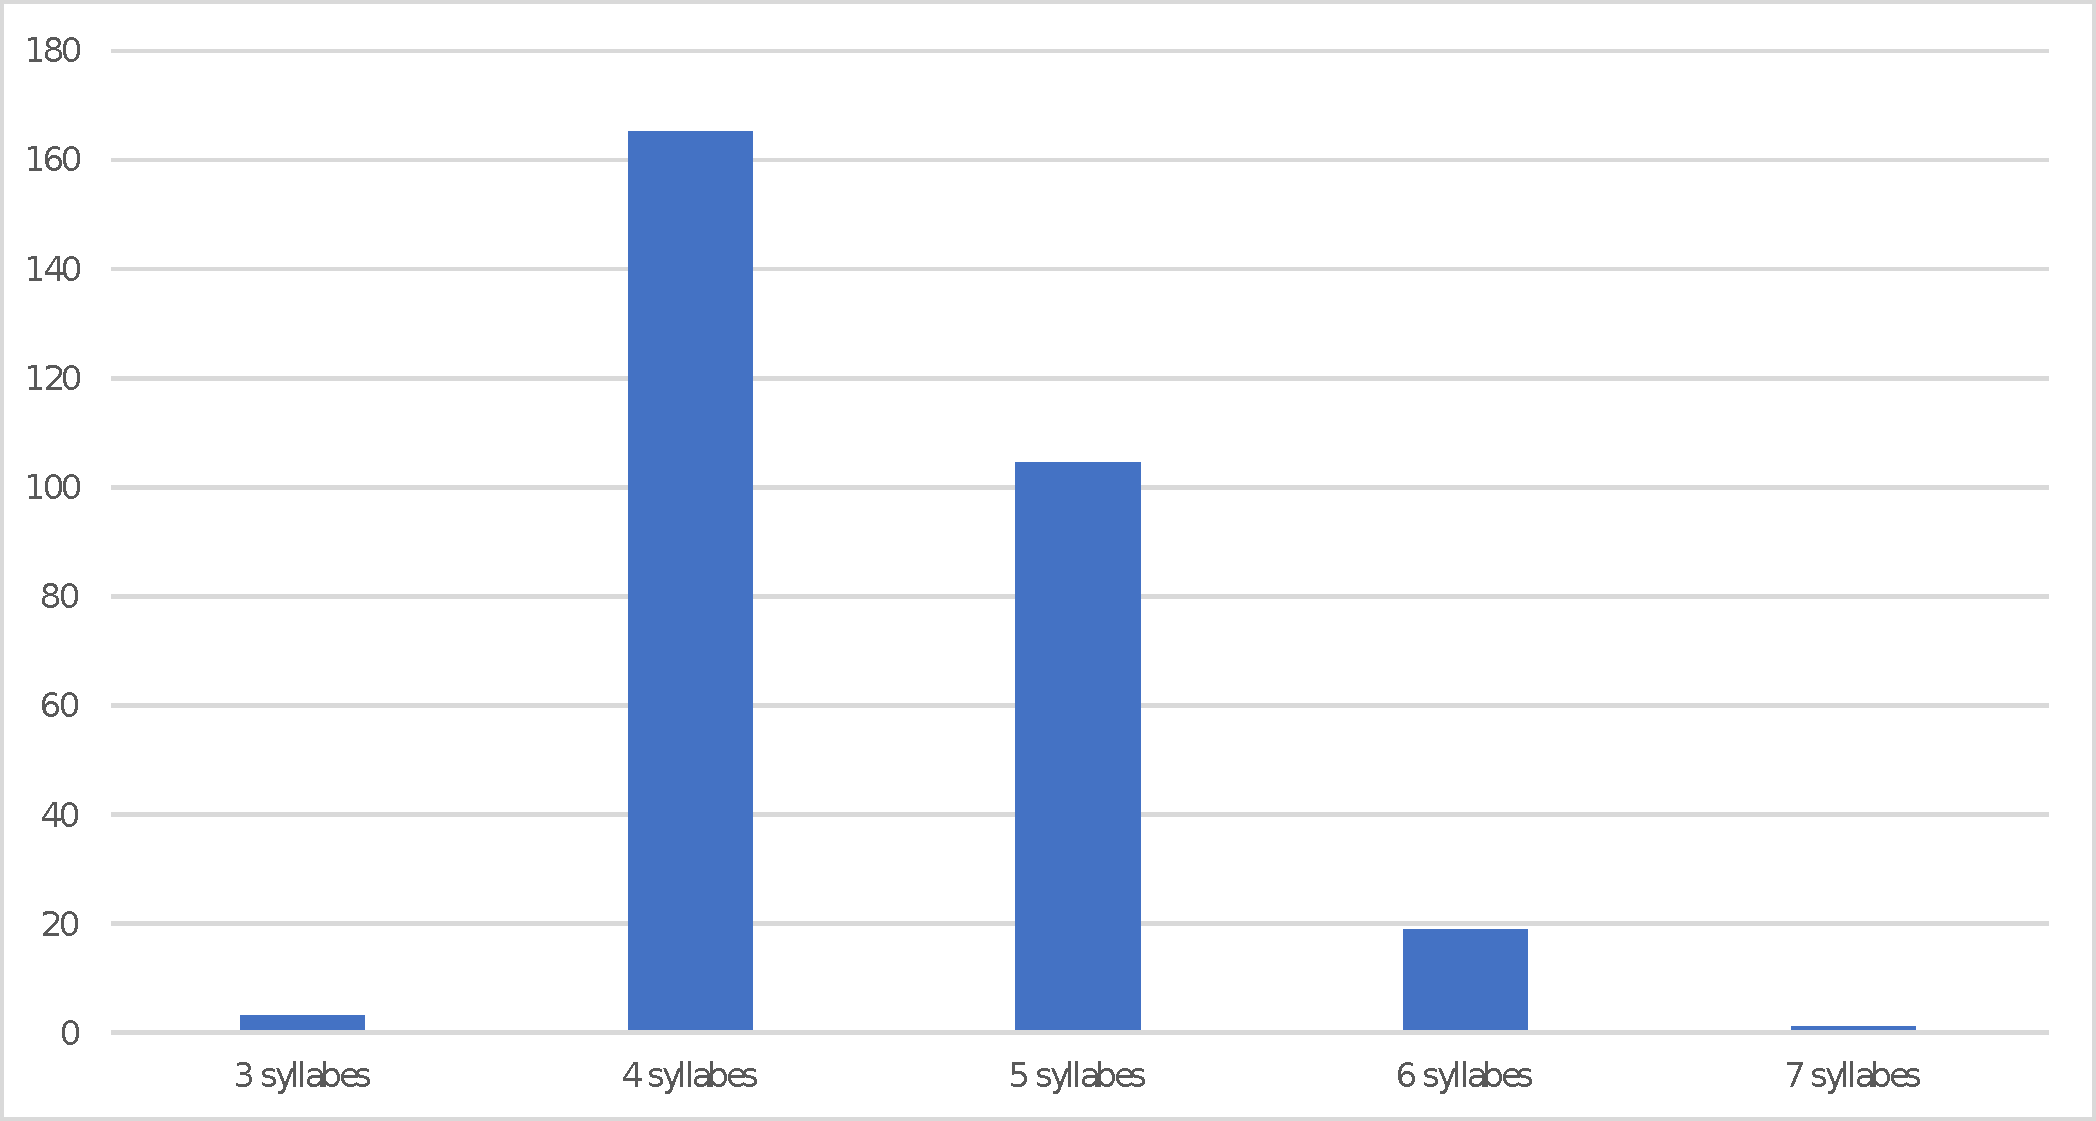
\includegraphics[height=.3\textheight]{figures/montermini-5.pdf}
\caption{Distribution des lexèmes en \textsc{-issimo} selon le
nombre de syllabes}
\label{fig:Montermini:5}
\end{figure}

\largerpage 
Dans l'interprétation de ces chiffres, il faut considérer que, puisque
-\textsc{issimo} se termine par voyelle, un dérivé quadrisyllabique
correspond à un dérivé trisyllabique en -\textsc{issime}, un
pentasyllabique à un quadrisyllabique, etc. En prenant en compte cette
différence, les deux formats les plus fréquents pour -\textsc{issime}
(trois et quatre syllabes) représentent 79,6\% des cas (cf. la figure
{fig:Montermini:4}), alors que pour -\textsc{issimo} les deux formats les plus fréquents
(quatre et cinq syllabes) représentent 91,4\% des cas. Il semble donc
que la contrainte de taille\is{constraint!size constraint} soit plus forte pour -\textsc{issimo} que
pour -\textsc{issime}, ce qui expliquerait la plus grande tendance de
cette construction à modifier les thèmes\is{stem} de base\is{base} sélectionnés en les
réduisant. Cette tendance que l'on observe pour -\textsc{issimo} a
cependant, également, une autre explication, complémentaire à celle que
je viens de proposer. Dans le tableau~\ref{ex:Montermini:20}, je récapitule le nombre de bases\is{base} qui
subissent une modification (réduction) du thème\is{stem} pour -\textsc{issime} et
-\textsc{issimo}, en le comparant au nombre de bases\is{base} totales qui
présentent les conditions pour une telle modification (rime en voyelle +
sifflante, rime en {[}i{]} + consonne, finale vocalique). Le premier
chiffre indique le nombre de bases\is{base} potentiellement modifiables, le
deuxième le nombre de bases\is{base} qui sont effectivement modifiées~:

\begin{table}[h]
\centering
\begin{tabular}[t]{lrrrr}
\lsptoprule
&\multicolumn{2}{c}{Bases modifiables} & \multicolumn{2}{c}{Bases modifiées}\\
\midrule
-\textsc{issime} &99 & (26,5\%) &28 & (28,3\%)\\
-\textsc{issimo} &128 & (43,5\%) &124 & (96,9\%)\\
\lspbottomrule
\end{tabular}
\caption{\label{ex:Montermini:20} Nombre de bases subissant une modicication}
\end{table}



Ces chiffres nous disent fondamentalement deux choses~: premièrement,
dans la dérivation en -\textsc{issimo} une base\is{base} potentiellement
modifiable est quasi systématiquement modifiée~; deuxièmement, dans
cette dérivation les bases\is{base} qui présentent une structure segmentale
compatible avec une réduction (et donc un amalgame avec l'exposant)
sont surreprésentées par rapport à celle en -\textsc{issime}, pour
laquelle nous pouvons considérer que la distribution des bases\is{base},
principalement sélectionnées sur base catégorielle et sémantique, est
aléatoire du point de vue phonologique\footnote{Le nombre de bases\is{base}
  potentiellement modifiables est même surestimé dans le tableau~\ref{ex:Montermini:20} pour
  -\textsc{issime}, puisqu'ici aucune distinction n'est faite entre les
  bases\is{base} bisyllabiques et les bases\is{base} plus que bisyllabiques qui sont les
  seules, selon Plénat, qui peuvent subir un effacement d'une rime
  complexe.}. Cette surreprésentation est justement due à la faible
sélection qu'opère -\textsc{issimo} sur ses bases\is{base} du point de vue
catégoriel et sémantique, ce qui laisse la place pour que la phonologie
y joue un rôle plus important. Peu importe que \mbox{\textsc{-issimo}}
constitue, de ce point de vue, une construction non canonique -- la
plupart des affixes, en effet, privilégient les propriétés catégorielles
et sémantiques dans la sélection de leurs bases\is{base}. Ce que ces données, et
leur interprétation, mettent en lumière, en effet, est une des voies que
la morphologie peut prendre dans la conventionnalisation des propriétés
(dans ce cas formelles) qui sont associées à ses constructions.

Pour conclure, on peut considérer que les contraintes\is{constraint!formal} formelles
attachées à la construction en -\textsc{issimo} sont les suivantes~: le
dérivé doit avoir la forme {[}Xisimo{]} \textgreater{} {[}XVsimo{]} (où
les formes possibles pour l'exposant sont hiérarchisées)~; le dérivé
doit comporter quatre ou cinq syllabes ou, à défaut, six syllabes ou un
nombre supérieur. On peut également imaginer que les
contraintes\is{constraint} catégorielles et sémantiques de sélection de la base\is{base} sont
remplacées par des contraintes\is{constraint} de sélection formelle que l'on peut
formuler et ordonner ainsi~:

% removed, not an example (21)

\largerpage
Une base\is{base} optimale pour un dérivé en -\textsc{issimo~}:

\begin{itemize}
\item[---] est bi- ou trisyllabique~;

\item[---] se termine par un {[}i{]} ou par une séquence {[}i{]}+sifflante~;

\item[---] est plus que trisyllabique et contient une séquence {[}i{]}+sifflante à
la deuxième ou à la troisième syllabe~;

\item[---] se termine par un {[}i{]} suivi d'une autre consonne~;

\item[---] se termine par une voyelle différente de {[}i{]}, suivie ou non d'une
sifflante.
\end{itemize}

Comme on le voit, les contraintes\is{constraint} qui occupent une place moins élevée
dans la hiérarchie manifestent des relâchements d'une des propriétés
spécifiées par les deux premières, soit sur le nombre de syllabes, soit
sur le timbre de la voyelle, soit sur la nature de la consonne de la
rime.

Pour rappel, j'ai considéré plus haut que les constructions en 
\textsc{-issime}, de leur côté, sont soumises, du point de vue de la
sélection des bases\is{base}, à des contraintes\is{constraint} catégorielles et sémantiques
semblables à celles qui opèrent pour les autres constructions affixales
canoniques. Du point de vue segmental, cette construction spécifie
uniquement que le dérivé doit avoir la forme {[}Xisim{]}~; du point de
vue prosodique, si des contraintes\is{constraint} de taille\is{constraint!size constraint} existent, elles sont
soumises aux contraintes\is{constraint} de fidélité\is{constraint!faithfulness constraint} base-dérivé.

\section{Conclusion}\label{sec:montermini:4}

La prise en compte des écarts entre la forme attendue et celle
réellement observée des lexèmes morphologiquement complexes est un des
domaines dans lesquels la recherche en morphologie, sur le français et
sur d'autres langues, a le plus évolué dans les dernières décennies.
Ceci s'est traduit, d'une part, par la reconnaissance des lexèmes comme
des structures complexes auxquelles peuvent correspondre,
synchroniquement, plusieurs thèmes\is{stem}, des représentations formelles qui
sont irréductibles, mais connectées entre elles et organisées. Parmi les
opérations que la morphologie (dérivationnelle) met en place lors de
l'application d'une règle (ou construction) morphologique, il y a la
définition d'un radical\is{stem}, c'est-à-dire la forme à laquelle est appliquée
l'opération formelle spécifiée par la règle. Cette définition passe par
la sélection d'un des thèmes\is{stem} du lexème de base\is{base} et par d'éventuelles
modifications phonologiques de celui-ci. Une façon de modéliser cet
ensemble d'opération est de considérer qu'elles sont régies par un
ensemble de contraintes\is{constraint}, c'est-à-dire de spécifications des propriétés
qu'un lexème dérivé doit avoir. Les contraintes\is{constraint} peuvent être spécifiques
à une langue (ou même à un secteur de la langue) ou bien universelles~;
elles peuvent se renforcer mutuellement, ou bien se contredire, et dans
ce cas la forme réellement observée pour un dérivé sera déterminée par
la tendance à satisfaire une contrainte\is{constraint} ou une autre, avec des issues
potentiellement différentes lorsqu'une opération est appliquée à la même
base\is{base}. Les travaux qui se sont inspirés de ce modèle, cependant, se sont
principalement intéressés à la variation thématique et aux facteurs qui
en sont responsables~; la variation des exposants des constructions
morphologiques (qui correspond à ce qui traditionnellement était vu
comme l'allomorphie\is{allomorphy} affixale\is{allomorphy!affix allomorphy}), en revanche, a moins suscité leur
intérêt. Pourtant, j'ai proposé des arguments forts pour soutenir que
certains cas de variation formelle que l'on observe en dérivation ne
peuvent pas être traités en termes de variation thématique. Il faut donc
admettre que les exposants des constructions morphologiques peuvent
aussi être sujets à variation, une variation qui mérite d'être prise en
compte et, si possible, modélisée. Cela pose, tout d'abord, le problème
d'identifier clairement les cas de variation d'un exposant au sein de la
même construction des cas de constructions différentes qui,
éventuellement, peuvent avoir une sémantique proche et des exposants
formellement semblables. Pour considérer que deux formes sont des
variantes du même exposant, il faut qu'elles soient non seulement
proches et si possible liées par des relations phonologiques naturelles,
mais qu'elles apparaissent dans des lexèmes dérivés qui ont des
propriétés catégorielles et sémantiques semblables (c'est-à-dire qui
appartiennent à la même série), et surtout qu'elles soient en
distribution complémentaire ou du moins que leurs contextes d'apparition
soient clairement identifiables du point de vue phonologique. Pour
modéliser la variation des exposants morphologiques, j'ai proposé
d'étendre la notion de contrainte\is{constraint} non seulement à une propriété qui est
spécifique à une langue donnée, mais également à une construction
donnée. Les exposants des constructions morphologiques peuvent alors
être vus eux-mêmes comme des contraintes\is{constraint}, ou des ensembles de
contraintes\is{constraint}, qui interagissent avec les autres contraintes\is{constraint} en jeu dans
la formation des lexèmes complexes. Chaque «~allomorphe\is{allomorphy}~» d'un exposant
est donc une contrainte\is{constraint} qui, en tant que telle, peut être hiérarchisée
par rapport aux autres, ce qui rend compte de l'observation que
certaines de ces variantes jouent un rôle de défaut, alors que d'autres
émergent uniquement dans des conditions particulières\footnote{Un
  relecteur de l'article suggère, en alternative, de considérer qu'une
  construction peut comporter plusieurs variantes de l'exposant, dont le
  choix est déterminé par des contraintes\is{constraint} de sélection (un système, à
  mon sens, semblable à celui proposé par %
%Bonet \emph{et al.} 2007
\citealt{Bonet2007} %
%
 pour
  le créole haïtien et le catalan, qui prévoit, pour certains procédés
  morphologiques, l'existence d'un «~catalogue~» de variantes
  hierarchisées). Il est vrai que l'efficacité des contraintes\is{constraint} a été
  déjà montrée pour la sélection du thème\is{stem} dans les procédés
  morphologiques constructionnels %
%(cf. Plénat \& Roché 2014~; Boyé \&
%  Plénat 2015)
\citep[cf.][]{Plenat-Roche2014,Boye15}%
%Plénat-Roché
%
, et une telle hypothèse permettrait d'unifier l'analyse
  des deux. Cependant, il me semble qu'une telle hypothèse devrait être
  considérée, au mieux, comme une variante de l'hypothèse principale que
  je défends, pour au moins deux raisons~: i) dans certains cas, comme
  celui de -\textsc{phone}, le «~catalogue~» des exposants correspondrait
  à une simple liste de formes largement redondante (dans le cas en
  question {[}fɔn{]} précédé de n'importe quelle voyelle et possiblement
  de plusieurs consonnes)~; ii) cette hypothèse ne permettrait pas de
  capter l'interaction entre la forme du thème\is{stem} de la base\is{base} et l'exposant,
  un élément crucial de l'analyse proposée ici.}.

Afin d'illustrer le modèle que je propose, j'ai réalisé deux études de
cas de constructions morphologiques de naissance ou développement
récent. Ce travail se place, en effet, dans une approche extensive de la
morphologie, dans laquelle est essentielle la prise en compte d'un
nombre important de données et, si possible, de données qui manifestent
la pratique réelle de construction des mots par les locuteurs. C'est
pour cela que l'observation des nouvelles formations, néologismes,
occasionalismes, etc. est tout aussi importante, sinon plus, que
l'observation du lexique établi. Les deux constructions que j'ai
considérées sont la création de noms de locuteurs en -\textsc{phone} à
partir du nom d'une langue et la création de lexèmes avec un sens
génériquement appréciatif / superlatif en -\textsc{issimo}. La première
a la particularité de prendre comme bases\is{base} aussi bien des noms de langues
qui appartiennent à des réseaux lexicaux nombreux, et pour lesquels la
sélection est donc un enjeu, et des noms de langues qui n'entretiennent
aucun lien lexical, ou très peu, qui peuvent donc être sujets à des
modifications destinées à en faire de «~bons~» radicaux\is{stem} pour la
construction en question. La deuxième, à cause de sa valeur pragmatique,
définit peu de contraintes\is{constraint} catégorielles et sémantiques sur ses bases\is{base}
potentielles, qui sont, en revanche, plutôt sélectionnées sur une base
formelle, selon leur compatibilité avec les contraintes\is{constraint} segmentales qui
en définissent l'exposant. Chacune de ces deux constructions fait
également l'objet d'une comparaison. La dérivation en -\textsc{phone}
est comparée à la dérivation correspondante et cognate de lexèmes en
-\textsc{fono} en italien~; la dérivation en -\textsc{issimo} est
comparée à la dérivation, plus canonique, de superlatifs en
‑\textsc{issime} en français. Ces comparaisons mettent en lumière le
fait que des constructions formellement et sémantiquement similaires et
qui ont la même origine peuvent, dans des langues différentes ou dans la
même langue à des époques et pour des finalités différentes, développer
des spécifications phonologiques différentes, ce qui se traduit, dans le
cadre adopté ici, par des ensembles de contraintes\is{constraint} différentes et/ou
agencées différemment. Je prends ce constat pour une
démonstration du fait que l'exposant d'une règle morphologique
correspond simplement à l'association arbitraire entre un ensemble de
spécifications catégorielles et sémantiques et un ensemble de
contraintes\is{constraint!formal} formelles.

Le modèle de morphologie à contraintes\is{constraint} ouvre de nombreuses perspectives
de recherche et de connexions potentielles avec des modèles théoriques
proches (par exemple la Morphologie des Constructions\is{Construction Morphology}). S'il a été
jusqu'à présent appliqué presque uniquement au français, ce modèle
mériterait d'être testé sur d'autres langues et sur des ensembles de
données plus variés. Le travail que j'ai présenté constitue, je
l'espère, un premier pas dans cette direction.

\section*{Remerciements}

Je tiens à remercier Gilles Boyé,
  Michel Roché et Anna M. Thornton pour leur précieux commentaires qui
  m'ont permis d'améliorer considérablement le texte de cet article.


%\nocite{Apotheloz2003}
%\nocite{Aronoff1976}
%\nocite{Baroni2009}
%\nocite{blevins2009.OUP}
%\nocite{Bonami2014}
%\nocite{Bonami03a}
%\nocite{BonamiBoye2014}
%\nocite{Bonami2009b}
%\nocite{Bonet2007}
%\nocite{Booij10}
%\nocite{Boye15}
%\nocite{Burzio2002}
%\nocite{bybee06}
%\nocite{Bybee2013}
%\nocite{Corbin2001}
%\nocite{Dal2012}
%\nocite{DalGeorgette2016}
%\nocite{VilloingDavidLeroy2014}
%\nocite{Fradin2000}
%\nocite{Fradin03}
%\nocite{Fradin2009}
%\nocite{Hathout2009}
%\nocite{Hathout2008}
%\nocite{HathoutMonterminiTseng2013}
%\nocite{hathout2014.imm15}
%\nocite{Hathout09}
%\nocite{Koehl2012}
%\nocite{KoehlAurore2014}
%\nocite{Lasserre2016}
%\nocite{lasserre2014.cmlf}
%\nocite{Lignon2013}
%\nocite{Lignon2014}
%\nocite{Lignon09}
%\nocite{LignonStephanie2011}
%\nocite{Montermini2003}
%\nocite{Montermini10}
%\nocite{Montermini2015}
%\nocite{namer2013}
%\nocite{Perko2010}
%\nocite{Plenat2002}
%\nocite{Plenat2008b}
%\nocite{Plenat08}
%\nocite{Plenat09}
%\nocite{PlenatLignonSernaTanguy2002}
%\nocite{Plenat-Roche2014}
%\nocite{Rainer2003}
%\nocite{Roche2008}
%\nocite{Roche2009}
%\nocite{Roche10}
%\nocite{Roche2011b}
%\nocite{Roche2013}
%\nocite{roche2011.dumal}
%\nocite{RocheMichel2012}
%\nocite{Roche14}
%\nocite{Roche16}
%\nocite{Scalise1999}
%\nocite{Thornton1999}
%\nocite{Thornton2007b}


\section*{Annexe}

Le tableau~\ref{tab:annexe} liste tous les lexèmes en -\textsc{issimo} cités dans
l'article avec une indication de leur emploi, tel qu'il a pu être
identifié à partir des recherches effectuées. Si le lexème n'est suivi
d'aucune indication, cela signifie qu'il a été repéré dans un emploi en
discours et que sa signification correspond en gros au superlatif du
lexème de base\is{base}.

\begin{table}
\centering
\begin{tabularx}{\textwidth}{QQ}
\lsptoprule
Acquissimo (type de crédit immobilier)	&	Linguissimo (concours de langues)	\\
Agrandissimo (constructeur immobilier)	&	Locatissimo (site de location d'appartements)	\\
Altissimo (magasin d'équipement pour escalade)	&	Narcissimo	\\
Anglissimo	&	Numissima (entreprise de rachat de précieux)	\\
Apéritissimo (bar à apéritifs)	&	Naturissima (salon sur la nature)	\\
Apprentissimo (salon sur l'apprentissage)	&	Nutrissimo (jeu de société sur la nutrition)	\\
Authentissima (magasin de mobilier)	&	Olympissimo (jeu de société sur les Jeux Olympiques)	\\
Bébéssimo (site de produits pour enfants)	&	Optimissimo	\\
Bijoutissimo (site de vente de bijoux)	&	Optissimo (chaîne d'opticiens)	\\
Blingissimo (marque de bijoux)	&	Parfumissimo (slogan publicitaire, 1969)	\\
Caféissimo (huile au café)	&	Permissimo (site pour la récupération des points du permis de conduire)	\\
Caféssimo (site de vente de café)	&	Pizzassimo (sauce tomate pour pizza)	\\
Cinessimo (nom d'une carte de crédit qui comporte des réductions au cinéma)	&	Prépassimo (école préparatoire)	\\
Colissimo (service de colis de la Poste)	&	Promessimo (type de contrat immobilier)	\\
Courissimo (compétition de course à pied)	&	Ravissimo (machine à découper les raviolis)	\\
Dégueulassimo	&	Repassimo (pressing)	\\
Diorissima (parfum de la marque Dior)	&	Revenussimo (site de conseils financiers)	\\
Doctissimo (site de médecine)	&	Scientissimo (site d'activités scientifiques)	\\
Dodossimo (pyjama pour enfants)	&	Sélectissimo (club d'affaires)	\\
Drolissimo	&	Successimo	\\
Énormissimo	&	Successissimo	\\
Equissimo (salon de chevaux)	&	Tassimo (machine à café)	\\
Erotissimo (film, 1969)	&	Tennissimo (centre sportif)	\\
Espérantissimo (site d'espéranto)	&	Torticolissimo	\\
Formidablissimo	&	Urbanissimo (site d'urbanisme)	\\
Historissimo (librairie)	&	Valorissimo (agence immobilière)	\\
Incroyablissimo	&	Vélossimo (association cycliste)	\\
Investissimo (agence immobilière)	&	Vernissimo (slogan publicitaire, 1966)	\\
Jonglissimo (festival de jonglerie)	&	Vomissimo	\\
Jurissimo (cabinet d'avocats)	&		\\
\lspbottomrule
\end{tabularx}
\caption{Liste des lexèmes en \emph{-issimo}\label{tab:annexe}}
\end{table}
\il{French|)}
\il{Italian|)}
{\sloppy
\printbibliography[heading=subbibliography,notkeyword=this]
}


\end{document}
